\documentclass[9pt,a4paper,fleqn,german]{scrartcl}

% enc
\usepackage[T1]{fontenc}
\usepackage[latin1]{inputenc}

\usepackage{german}
\usepackage[german]{babel}

% tweaking f�r pdf 
\usepackage{ae}
\usepackage{a4}
%\usepackage{anysize}
\usepackage[left=1cm,top=1cm,right=1cm,nohead,nofoot]{geometry}
\pagestyle{empty}

% references
\usepackage[ps2pdf]{hyperref}
\usepackage{varioref}

% grafiken
\usepackage{graphicx}
%\usepackage{pictex}

% speziell symbole
\usepackage{latexsym}
\usepackage{amsmath}
\usepackage{amssymb}
\usepackage{mathbbol}
\usepackage{pxfonts}
\usepackage[small,compact]{titlesec}
\usepackage{float}

% itemstacking
\usepackage{atbeginend}
\AfterBegin{itemize}{ \addtolength{\itemsep}{-2ex}}
\AfterBegin{enumerate}{ \addtolength{\itemsep}{-2ex}}
\BeforeBegin{tabular}{ \vspace{-2ex} }
\AfterEnd{tabular}{ \vspace{-2ex} }
\BeforeBegin{figure}{ \vspace{-2ex} }
\AfterEnd{figure}{ \vspace{-2ex} }

% PPCHTEX
\usepackage{m-pictex}
\usepackage{m-ch-de}

\hypersetup{%
pdftitle = {CRT Formelsammlung},
pdfsubject = {Kurzzusammenfassung und Formelsammlung zum Kernfach "Chemische Reaktionstechnik", CBI, Erlangen},
pdfauthor = {Florian Enzenberger, Sebastian Werner},
pdfcreator = {GhostScript},
pdfproducer = {LaTeX}
}

% mehr zeuch aufs blatt
%\setlength{\textheight}{25cm}
%\setlength{\topmargin}{-1cm}
%\setlength{\parskip}{\baselineskip}
\addtolength{\parskip}{-1mm}
\setlength{\parindent}{0pt}

% brauchen latex2e
\NeedsTeXFormat{LaTeX2e}

% neue commands
\newcommand{\osum}{\sum \hspace*{-2.4ex}\vspace*{-1ex} \circ\hspace*{2.4ex}\vspace{1ex}}

\begin{document}

%zweispaltig mit �berschrift zentriert
\twocolumn[{\csname @twocolumnfalse\endcsname
{\centerline{ \Huge \sc Formelsammlung Chemische Reaktionstechnik I}}
{\centerline{ \it Florian Enzenberger, Friedrich Glenk, Daniel Ludwig, Matthias Pemsel \& Sebastian Werner, 2005 } }
{\centerline{ \bf Keinerlei Anspruch auf Vollst�ndigkeit oder Richtigkeit! }}
\vspace{1ex}
}]

\section{Basiswissen}
\subsection{Konventionen}
\begin{itemize}
\item Index $h = 1...L$ - Elemente
\item Index $i = 1...N$ - Komponenten / Spezies
\item Index $j = 1...M$ - Teilreaktionen
\item Exponent $m_i$ - Teilreaktionsordnung bezogen auf $A_i$ (St�ch. Koeffizient?!)
\item St�chimetrische Koeffizienten $\nu_i$. $\nu_i < 0$: Edukt, $\nu_i > 0$: Produkt
\item Elementkoeffient des Elements $h$ in Spezies $i$: $\beta_{hi}$
\item Geschwindigkeitskoeffizient $k$ $\left[ \frac{mol}{l \cdot s}\right]$
\item Bildungs- bzw. Verbrauchsgeschwindigkeit $R$ \emph{ Rate of formation / deplition}
\item Reaktionsgeschwindigkeit $r$
\end{itemize}

\subsection{Definitionen}
\begin{itemize}
\item \emph{ Extensive} Terme: Variablen eines Systems, welche sich bei Teilung des Systems in zwei Teilsysteme �ndern. Bsp: $V$, $m$, $n$
\item \emph{Intensive} Terme: Variablen eines Systems, die bei Teilung des Systems in Teilsysteme konstant bleiben. Bsp: $T$, $p$, $\rho$
\item Extensive Variablen k�nnen durch Normierung �ber $m$ oder $V$ zu \emph{Pseudo-Intensiven} Variablen umgewandelt werden.
\item Massenerhaltung 
\[ \sum_{i=0}^{N} \nu_i M_i = 0 \]
\end{itemize}

\subsubsection{Reaktionslaufzahl}
  \begin{displaymath}
  \fbox{$ \displaystyle   \displaystyle   \displaystyle   \xi = \frac{n_i - n_{i0}}{\nu_i} $}
  \end{displaymath}
  \begin{itemize}
  \item $\xi = 0$: Reaktionsbeginn
  \item $\xi = 1$: Reaktionsende
  \item $c_i = c_{i0} + \nu_i \lambda$
  \item $m_i = m_{i0} + M_i \nu_i \xi$
  \item $n_i = n_{i0} + \nu_i \xi$
  \end{itemize}

\subsubsection{Umsatz}
  \begin{itemize}
  \item \[ \fbox{$ \displaystyle   \displaystyle   \displaystyle    \mbox{Umsatz} = \frac{\mbox{Anteil an bereits Reagierter Komponente}}{\mbox{Anfangsmenge der Komponente}}$} \]
  \item Diskontinuierlich
  \[ X_i = \frac{n_{i0} - n_i}{n_{i0}} = - \frac{\sum_{j=1}^{M} \nu_{ij} \xi_i}{n_{i0}} \]
  \item Kontinuierlich
  \[ \fbox{$ \displaystyle   \displaystyle   \displaystyle    X_i = \frac{\dot{n}_{i0} - \dot{n}_i}{\dot{n}_{i0}} $} \]
  \end{itemize}

\subsubsection{Ausbeute}
  \begin{itemize}
  \item \[ \fbox{$ \displaystyle   \displaystyle   \displaystyle    \mbox{Ausbeute} = \frac{\mbox{Menge an gebildetem Produkt k}}{\mbox{Menge an zugegebener, limitierender Komponente i}} $} \]
  \item Diskontinuierlich
  \[ Y_{ki} = \frac{\frac{n_k - n_{k0}}{\nu_k}}{\frac{n_{i0}}{\nu_i}} = \frac{n_k - n_{k0}}{n_{i0}} \frac{\left|\nu_i\right|}{\left|\nu_k\right|} \]
  \item Kontinuierlich 
  \[ Y_{ki} = \frac{\dot{n}_k - \dot{n}_{k0}}{\dot{n}_{i0}} \frac{\left|\nu_i\right|}{\left|\nu_k\right|} \]
  \end{itemize}

\subsubsection{Selektivit�t}
  \begin{itemize}
  \item \[ \fbox{$ \displaystyle   \displaystyle   \displaystyle    \mbox{Selektivit�t} = \frac{\mbox{Menge an gebildetem Produkt k}}{\mbox{Menge an umgesetztem Reaktanden i}} $} \]
  \item Diskontinuierlich
  \[ S_{ki} = \frac{n_k - n_{k0}}{n_{i0} - n_i} \frac{\left|\nu_i\right|}{\left|\nu_k\right|} = \frac{Y_{ki}}{X_i} \]
  \item Kontinuierlich
  \[ S_{ki} = \frac{\dot{n}_k - \dot{n}_{k0}}{\dot{n}_{i0} - \dot{n}_i} \frac{\left|\nu_i\right|}{\left|\nu_k\right|} = \frac{Y_{ki}}{X_i} \]
  \end{itemize}

\subsubsection{Reaktorkenngr��en}
\begin{itemize}
\item Produktivit�t
\[ L = \dot{n}_k \]
\item Querschnittsbelastung
\[ G = \frac{m}{A t} \]
\item Raum-Zeit-Ausbeute
\[ STY = \frac{L}{V} = \frac{\dot{n}_k}{V} \]
\end{itemize}


\section{Beschreibung einfacher Reaktionen}
\subsection{Potenzansatz - Power Law Expressions}
  \[ \fbox{$ \displaystyle  \displaystyle   r = k c_1^{m_1} c_2^{m_2} = \frac{1}{\nu_i}\frac{dc_i}{dt} $} \]
  bzw. allgemeiner:
  \[ r = k \prod_i^N c_i^{m_i} \]

\subsection{Temperaturabh�ngigkeit einer Reaktion - {\sc Arrhenius}-Law}
  \begin{itemize}
  \item {\sc Arrhenius}-Gleichung 
  \[ \fbox{$ \displaystyle k = k_0 \exp\left(-\frac{E}{RT}\right) $} \]
  \item im {\sc Arrhenius}-Plot: $\ln k$ gegen $\frac{1}{T}$ wegen
  \[ \ln k = - \frac{E}{R} \frac{1}{T} + \ln k_0 \]
  \item Aktivierungsenergie $E$ liegt normalerweise im Bereich $40...200\, \frac{kJ}{mol}$
  \item Sto�faktor $k_0 \left[\frac{mol^{1-m}}{s}\right]$
  \item Faustregel: Temperaturerh�hung um $10\,K$ verdoppelt Reaktionsgeschwindigkeit!
  \end{itemize}

\subsection{Definition der Reaktionsgeschwindigkeit}
  \begin{itemize}
  \item \[ r^* = \frac{1}{\nu_i} \frac{dn_i}{dt} = \frac{d\xi}{dt} \]
  Achtung: Extensive Gr��e!
  \item Homogene Reaktionen (Normierung auf Reaktionsvolumen bzw. -Masse)
  \[ \fbox{$ \displaystyle  \displaystyle   \frac{r^*}{V} = \frac{1}{V}\frac{d\xi}{dt} $} \quad \left[\frac{mol}{m^3\,s}\right] \qquad \fbox{$ \displaystyle  \displaystyle   \frac{r^*}{m} = \frac{1}{m}\frac{d\xi}{dt} $} \quad \left[\frac{mol}{kg\,s}\right] \]
  \item Heterogene Reaktionen (Normierung auf Katalysatoroberfl�che bzw. -Masse)
  \[ \fbox{$ \displaystyle  \displaystyle   \frac{r^*}{A} = \frac{1}{A}\frac{d\xi}{dt} $} \quad \left[\frac{mol}{m^2\,s}\right] \qquad \fbox{$ \displaystyle  \displaystyle   \frac{r^*}{m_{cat}} = \frac{1}{m_{cat}}\frac{d\xi}{dt} $} \quad \left[\frac{mol}{kg\,s}\right] \]
  \item Sonderfall: Reaktionsvolumen $V = const$
  \[ \fbox{$ \displaystyle  \displaystyle   r = \frac{1}{\nu_i} \frac{dc_i}{dt} $} \]
  \item Achtung: Reaktionsgeschwindigkeit wird auf eine \emph{Reaktion} bezogen, die Bildungs- bzw. Verbrauchsgeschwindigkeit wird hingegen auf eine \emph{Spezies} bezogen!
  \end{itemize}

\subsection{Bildungs- bzw. Verbrauchsrate}
\[ \fbox{$ \displaystyle  \displaystyle   R_i = \frac{dc_i}{dt} = \sum_{j=1}{M} \nu_{ij} r_i $} \]
bei $V = const$

\subsection{Reaktionen 1. Ordnung}
Umwandlung eines Molek�ls in ein anderes: \[ \chemie{A_1} \chemie{GIVES} \chemie{A_2}\]
\[ \fbox{$ \displaystyle  \displaystyle   R = \frac{dc_1}{dt} = \nu_1 r = - k\cdot c_1 $} \]

\subsection{Reaktionen 2. Ordnung}
\subsubsection{2 Gleichartige Reaktanden}
\[ \chemie{2 A_1}  \chemie{GIVES} \chemie{A_2} \]
\[ \fbox{$ \displaystyle  \displaystyle   R = \frac{dc_1}{dt} = - 2 r = - 2 k c_1^2 $} \]
\subsubsection{2 Ungleiche Reaktanden}
\[ \chemie{A_1} \chemie{PLUS} \chemie{A_2} \chemie{GIVES} \chemie{A_3}\]
\[ r = - \frac{dc_1}{dt} = - \frac{dc_2}{dt} = k c_1 c_2 \quad \leadsto \quad \fbox{$ \displaystyle  \displaystyle   R = - k c_1 c_2 $} \]
Spezialfall: Reaktion Pseudo 1. Ordung $\leftrightarrow$ Ein Reaktand liegt in unendlicher Konzentration vor.\\
In diesem Fall: $c_2 = c_{20}$
\[ \fbox{$ \displaystyle  \displaystyle   \frac{dc_1}{dt} = - \underbrace{k c_{20}}_{= k_{eff}} c_1 = - k_{eff} c_1 $} \quad \mbox{bei } c_{20} \gg c_{10} \]


\section{Wichtige Gro�technische Prozesse}
\subsection{Schwefels�ureherstellung}
\begin{enumerate}
\item Verbrennung von Schwefel zu $SO_2$
\item Oxidation von $SO_2$ $\quad \chemie{SO_2} \chemie{EQUILIBRIUM}{V_2O_5}{400..600�C} \chemie{SO_3} \qquad \Delta H_R = - 99 \frac{kJ}{mol} $
\item $SO_3$-Absorption an Wasser $\quad \chemie{SO_3} \chemie{PLUS} \chemie{H_2O} \chemie{GIVES} \chemie{H_2SO_4} \qquad \Delta H_R = - 132,5 \frac{kJ}{mol} $
\end{enumerate}

\subsection{Methanolherstellung}
\[ \chemie{CO} \chemie{PLUS} \chemie{H_2} \chemie{EQUILIBRIUM} \chemie{CH_3OH} \qquad \Delta H_R = - 92 \frac{kJ}{mol} \]

\subsection{Ammoniakherstellung}
Der aufw�ndigste Teil ist hierbei die Bereitstellung des Synthesegases!
Dieses wird in mehreren Schritten ausgehend von Methan hergestellt:
\subsubsection{Steam-Reforming}
\[ \chemie{CH_4} + \chemie{H_2O} \chemie{EQUILIBRIUM} \chemie{CO} + \chemie{3 H_2} \qquad \Delta H_R = 206 \frac{kJ}{mol} \]
Stark endothermer Prozess, welcher im Radiation-Convection-Oven durchgef�hrt wird.

\subsubsection{Luftzugabe - Autothermal-Reforming}
\[ \chemie{H_2} + \chemie{O_2}_{Luft} \chemie{EQUILIBRIUM} \chemie{H_2O} \]
Dient ihn Stand-Alone-Anlagen dazu, den Stickstoff bereitzustellen. Der Sauerstoff wird in einer Knallgasreaktion verbraucht.
Die ebenfalls anwesenden Edelgase sind inert. In integrierten Anlagen mit Luftzerleger wird oftmals direkt $N_2$ zugegeben.

\subsubsection{Wasser-Gas-Shift}
\[ \chemie{CO} + \chemie{H_2O} \chemie{EQUILIBRIUM} \chemie{CO_2} + \chemie{H_2} \qquad \Delta H_R = -41 \frac{kJ}{mol} \]
Hier ist zur Verschiebung des Gleichgewichts eine �berm�ssige Zugabe von Wasser notwendig. Da die Reaktion leicht exotherm ist,
muss die Temperatur niedrig gehalten werden. Technisch wird meist ein High-Temp und ein Low-Temp Reaktor mit intermedi�rer K�hlung realisiert.

\subsubsection{Entfernung von $CO_2$}
Das entstandene $CO_2$ wird durch das {\sc Rectisol}-Absorptionsverfahren (Methanol als Absorpt bei sehr niedrigen Temperaturen $-75 �C$ und $25 bar$).

\subsubsection{Methanisierung}
\[ \chemie{CO} + \chemie{3 H_2} \chemie{EQUILIBRIUM} \chemie{CH_4} + \chemie{H_2O} \qquad \Delta H_R = - 206 \frac{kJ}{mol} \]
Die hoch Exotherm bei 620K / 30bar wird durchgef�hrt um das Katalysator-Gift $CO$ in ppm-Bereich abzusenken.

\subsubsection{Ammoniaksynthese}
\[ \chemie{N_2} \chemie{PLUS} \chemie{H_2} \chemie{EQUILIBRIUM} \chemie{2 NH_3} \qquad \Delta H_R = - 91 \frac{kJ}{mol} \]
Optimierungsproblem zwischen Temperatur (hoch: wenig $NH_3$, niedrige: Reaktionsgeschwindigkeit sinkt) und Druck ($100-300 bar$).\\
Als Katalysatoren dienen, sehr �hnlich denen von Haber/Bosch gefundenen, immer noch Eisen-basierte Mischungen.\\
In der Praxis w�hlt man 675K am Inlet und 720..770K am Outlet bei 100..300bar. Auf Grund der Exothermie ist eine K�hlung notwendig.
Hier w�hlt man meist Hordenreaktoren mit direkter oder indirekter K�lung.\\
Durch die geringen Ums�tze (20..30\%) wird das Synthesegas im Loop gefahren. Hierzu wird das entstandene $NH_3$ kondensiert und abgezogen, w�hrend der Rest r�ckgef�hrt wird. Technisch bieten sich verschiedenste Varianten der Verschaltung.


\subsection{Steamcracking}
\begin{itemize}
\item Das Streamcracken dient der Herstellung von kurzkettigen Alkenen aus unreaktiven Alkanen
\item Der Dampf dient als Verd�nnungsmedium, um h�here Ums�tze (vgl {\sc Le Chatelier}) zu erzielen
\item Streamcracking erzeugt einen {\it Zoo von Produkten}, deren Anteile je nach Betriebsbedingung stark variieren
\end{itemize}
\subsubsection{Thermodyn. Aspekte}
\begin{itemize}
\item Steamcracking ist stark endotherm $\rightarrow$ Hohe Temperaturen
\item Je h�her die Temperatur, desto kurzkettiger die Alkene
\end{itemize}
\subsubsection{Mechanismus}
Der Prozess folgt einer Radikalkettenreaktion ohne Katalysator.
Start:
\[ H_3C\,CH_3 \chemie{GIVES} 2\, H_3C\cdot \]
Fortpflanzung:
\[ H_3C\cdot + H_3C\,CH_3 \chemie{GIVES} H_3C\,\dot{C}H_2 \]
\[ H_3C\,\dot{C}H_2 \chemie{GIVES} H_2C=CH_2 + H\cdot \]
\[ H\cdot + H_3C\,CH_3 \chemie{GIVES} H_3C\,\dot{C}H_2 \]
Abbruch: Rekombination beliebiger Radikale.
\subsubsection{Kinetik}
Streamcracken ist Reaktion 1. Ordnung: $r \sim p_{Feed}$.\\
Aber: hoher $p_{Feed}$ beg�nstig Zweitreaktionen und die Bildung von Verkokungsprodukten. Zudem wird die Einstellung des Gleichgewichts nicht beg�nstigst.\\
$\rightarrow$ Partialdruck und Umsatz gering halten! Reaktivit�t beim Cracken steigt mit C-Zahl. Somit: Kurze Kontaktzeiten und schnelles quenchen.
\subsection{Industrielle Ausf�hrung}
Aus den Vor�berlegungen folgt:
\begin{itemize}
\item hoher W�rme�bergang, hohe Temperatur
\item geringer Partialdruck
\item kurze Kontakt-/Verweilzeiten
\item schnelles Quenchen, um Zusammensetzung zu erhalten
\end{itemize}
Daraus ergibt sich das Bauprinzip des Radiation-Convection-Ovens.
\begin{itemize}
\item Vorw�rmen (auf $~ 870K$) von Naphta ($C_8...C_{10}$-Schnitt) in der Konvektionszone
\item Kurze Kontaktzeit ($< 1s$) bei sehr hoher Temperatur ($~ 1120K$) in der Radiation-Zone
\item Quenchen auf etwa $700K$ 
\item $Re$-Zahlen von $10^6$, L�nge der Rohre 50-200m.
\end{itemize}

\subsection{Fischer-Tropsch-Synthese}
Das in den 20er Jahren von Fischer und Tropsch am Kaiser-Wilhelm-Institut entwickelte Verfahren dient dazu aus Synthesegasen beliebiger Herkunft (Erdgas, Kohle, Biomasse, ...) Aliphatische Kohlenwasserstoffe zu erzeugen.

\subsubsection{Mechanismus}
\[ CO + 2 H_2 \chemie{GIVES}{Fe,Co}{200-350�C\\25bar} -(CH_2)_n- + H_20 \qquad \Delta H_R = -152\frac{KJ}{mol}\]
Auch wenn der Mechanismus nicht in letzter Wahrheit gekl�rt ist, wird wohl folgendes ablaufen:
\begin{itemize}
\item Adsorption $CO$
\item Dissoziation $CO$
\item Dissoziative Adsorption von $H_2$
\item Transfer $2 H$ an Kohlenstoff
\item Transfer von $2 H$ an Sauerstoff
\item Desorption von $H_2O$
\item Bildung einer $C-C$-Bindung
\item Desorption des Alkans
\end{itemize}
Hierbei bestimmt die Kennzahl $\alpha$ die Kettenl�nge:
\[ \fbox{$ \displaystyle \alpha = \frac{k_{growth}}{k_{growth}+k_{diss.+hydr.}} $} \]
$\alpha$ ist abh�ngig von Temperatur, $CO/H_2$-Verh�ltnis, Druck, Art des Katalysators, Promotoren.\\
Bei $\alpha < 0,85$ werden eher $C_5..C_{10}$ erzeugt, bei $\alpha > 0,85$ eher Wachse.

\subsubsection{Katalysatoren}
F�r die FT bieten sich Eisen, Cobalt, Nickel und Ruthenium als Katalysatoren an.
In der Praxis werden aber nur Eisen und Cobalt verwendet, da die Gefahr der Vergiftung bei Nickel hoch ist (Carbonyl-Nickel!) und Ruthenium als seltenes, teures Material nicht in gro�en Anlagen eingesetzt werden kann.

\subsubsection{Reaktoren}
Grunds�tzlich muss bedacht werden, dass die Reaktion exotherm ist. Somit muss die entstehende W�rme zuverl�ssig abgef�hrt werden, da Hot-Spots zu einer schnellen Desaktivierung des Katalysators f�hren und zudem vermehrt Methan gebildet wird.
Man unterscheidet zwischen Low-Temp und High-Temp FT-Synthese:
\begin{table}[H]
\begin{tabular}{l|c|c} 
                & \bf Low-Temp   & \bf High-Temp \\ \hline
Temperatur	& 220..250	& 330..350 \\
Methan	\%	& 2..5	& 10..11 \\
$C_2$..$C_4$ Olefine & 5 & 24..27 \\
$C_2$..$C_4$ Paraffine & 5..7 & 7..10 \\
$C_5$..$C_11$ Benzin & 18..22 & 37..40 \\
$C_12$..$C_18$ Diesel & 14..15 & 5..11 \\
$> C_19$ & 41..52 & 4..8 \\
Hydrophile & 3 & 5..6 \\
Org. Hydrophob Sre. & traces & 1 \\
\end{tabular}
\end{table}

Als Reaktoren werden in der Praxis Realisiert.
\paragraph{Synthol}
Zirkulierende Wirbelschicht f�r HT-FT-Synthese.
Kennzeichen:
\begin{itemize}
\item Hohe Gasgeschwindigkeit
\item Kleine Katalysator-K�rner ($100 \mu m$-Bereich)
\item Zwei K�hlzonen im Riser
\item Klassisches Verfahren seit 1955
\end{itemize}

\paragraph{Sasol Advanced Synthol}
Station�rer Wirbelschichtreaktor f�r HT-FT-Synthese.
\begin{itemize}
\item Wesentlich einfachere Konstruktion
\item Geringerer Druckverlust
\item H�here Kapazit�t
\item Katalysator permanent im Reaktor
\end{itemize}

\paragraph{ARGE}
Festbett-Multitubular-Reaktor f�r LT-FT-Synthese.
\begin{itemize}
\item Geringer Umsatz pro Durchlauf, um moderates Temperatur und Konzentrationsprofil entlang des Rohres zu realisieren
\item W�rmeabfuhr durch Wasserverdampfung
\item Aktuell 2050 Rohre mit 12m L�nge bei 5cm Innendurchmesser
\end{itemize}

\paragraph{Slurry}
Slurry aus hochsiedenden Wachsen, in welchem Katalysator "rumschwimmt" und Gas eingeblasen wird.
\begin{itemize}
\item Einfache Bauweise
\item Isothermie durch K�hlschlangen
\item Geringer Druckverlust
\item Optimale Umgebung f�r Katalysator
\item Kontinuierlicher Wechsel des Katalysators m�glich
\end{itemize}

\subsubsection{Bedeutung}
Um einen Schnitt mit m�glichst wertvollen Produkten zu erzielen, muss eine hohe Selektivit�t eingestellt werden.\\
Hier kann das Beispiel der 1-Olefine genannt werden, welche einen 6x h�heren Marktpreis als Benzin erzielen. Diese
k�nnen optimal in einer Wirbelschicht mit Fe-Katalysator erzeugt werden (70\% 1-Olefine in $C_5$..$C_{10}$-Fraktion!).\\
Besonders reizvoll ist die hohe Reinheit der Produkte, welche die einzelnen Fraktionen f�r Einsatz in Polymer-Herstellung oder
auch f�r Hochleistungskraftstoffe ("Shell-V-Power") oder Ultra-Low-Sulfur-Diesel pr�destiniert. Hierzu wird z.B. eine LT-FT genutzt, hinter
welcher ein Hydrocracker geschaltet ist, so das bis zu 80\% Ausbeute erzielt werden kann.\\
Eine andere Variante ist, statt Erdgas als LPG/LNG zum Markt zu transportieren, einfach eine FT zu nutzen.


\section{Konzentrationsverl�ufe spezieller Reaktionen}
\subsection{Reversible Reaktion 1. Ordnung}
\[ \chemie{A_1} \chemie{EQUILIBRIUM}{k1}{k2} \chemie{A_2} \]
\[ R_1 = \frac{dc_1}{dt} = - k_1 c_1 + k_2 c_2 \]
\[ K = \frac{c_2^*}{c_1^*} = \frac{c_{10} - c_1^*}{c_1^*} \]
$^*$ bedeutet: Gleichgewichtskonzentration
\[ \ln \frac{c_1 - c_1^*}{c_{10} - c_1^*} = - (k_1+k_2)t \]
{\bf Hier Bild  Konzentrationsverlauf}

\subsection{Parallelreaktion}
\[ \chemie{A_1} \chemie{GIVES}{k_1} \chemie{A_2} \hbox{gleichzeitig}  \chemie{A_1} \chemie{GIVES}{k_2} \chemie{A_3} \]
\[ \frac{dc_1}{dt} = - (k_1 + k_2) c_1 \quad \leadsto \quad \frac{c_1}{c_{10}} = \exp\left[-(k_1+k_2)t\right] \]
{\bf Hier Bild  Konzentrationsverlauf}
Hier auch wichtig: Globale Selektivit�t \[ S = \frac{c_2 - c_{20}}{c_3 - c_{30}} = \frac{k_1}{k_2} \]

\subsection{Folgereaktionen}
\[\chemie{A_1} \chemie{GIVES}{k_1} \chemie{A_2} \chemie{GIVES}{k_2} \chemie{A_3}\]

\subsubsection{Bildungsgeschwindigkeiten}
\[ R_1 = \frac{dc_1}{dt} = -k_1 c_1 \quad \leadsto \quad c_1(t) = c_{10} \exp(-k_1t) \]
\[ R_2 = \frac{dc_2}{dt} = k_1c_1 - k_2c_2 \]
\[ R_3 = \frac{dc_3}{dt} = k_2 c_2 \]
\subsubsection{Quastistationarit�tsprinzip nach {\sc Bodenstein}}
Wenn $\frac{dc_2}{dt}$ sehr klein (wegen $k_2 \gg k_1$), dann ist die Konzentration der Zwischenprodukte (nach einer Induktionszeit) \emph{quasistation�r}.
Daraus folgt: \fbox{$ \displaystyle \frac{dc_2}{dt} \approx 0$}
\subsubsection{Konzentrationsverl�ufe}
\begin{enumerate}
\item $k_1 = k_2$
\item $k_1 = 20 k_2 \qquad k_1 \gg k_2$
\item $20 k_1 = k_2 \qquad k_1 \ll k_2$
\end{enumerate}
\subsubsection{Anwendung des {\sc Bodenstein}-Prinzips}
\[ \frac{dc_2}{dt} = k_1c_1 - k_2 c_2 \approx 0 \quad \leadsto k_1 c_1 = k_2 c_2 \]
mit
\[ c_1 = c_{10} \exp\left(-k_1t\right) \quad \leadsto \quad c_2 = \frac{k_2}{k_1} c_{10} \exp\left(k_1\right) \]


\section{St�chiometrie chemischer Reaktionen}
\subsection{Allgemeines}
$N$ Komponenten: $A_1...A_N$ chemische Spezies\\
Schl�sselkomponenten: Mol�nderungen m�ssen bekannt / messbar sein, um eine Aussage �ber die Mol�nderungen der anderen Komponenten zu bekommen.
Schl�sselreaktionen:
\[ \frac{dc_i}{dt} = \sum_{j=1}^{M} \nu_{ij} r_j \]
Anzahl der Mole eines Elements:
\[ b_h = \sum_{i=1}^N \beta_{hi} n_i \quad \sum_{i=1}^N \beta_{hi} \Delta n_i = 0\]

\subsection{Element-Spezies-Matrix}
Bsp. Methanolherstellung.
\begin{table}[H]
\begin{tabular}{|ccc|ccc|cccc|} \hline
\multicolumn{3}{|c|}{ } & \multicolumn{7}{|c|}{$N = 7$} \\ \hline
$h$ & Elem & $i \rightarrow$    & 1 & 2 & 3 & 4 & 5 & 6 & 7 \\
    &      & Spez $\rightarrow$ & $C$ & $CH_4$ & $H_2O$ & $H_2$ & $CO$ & $CO_2$ & $ C_2H_6$\\ \hline
1   & C    &                        & 1 & 1 & 0 & 0 & 1 & 1 & 2 \\
2   & H    &                        & 0 & 4 & 2 & 2 & 0 & 0 & 6 \\
3   & O    &			  & 0 & 0 & 1 & 0 & 1 & 2 & 0 \\ \hline
\multicolumn{3}{|l|}{$L = 3$} & \multicolumn{3}{|c|}{gebunden} & \multicolumn{4}{|c|}{frei} \\ \hline
\end{tabular}
\end{table}
Matrix B hat den Rang $R_{\beta}=3$. \\
Anzahl der Spezies meist gr��er als Anzahl der Elemente. Dann miest $R_{\beta} = L$.\\
\[ R = N - R_{\beta} \]
\begin{itemize}
\item $R$ Zahl der Schl�sselkomponenten - Freie Unbekannte
\item $R_{\beta}$ gebundene Unbekannte - werden berechnet
\item Anzahl Schl�sselreaktionen = Anzahl Schl�sselkomponenten
\end{itemize}
Das System kann von unten gel�st werden: $\Delta n_{H_2} = - \Delta n_{CO} - 2 \Delta n_{CO_2}$ etc.

\subsection{Ermittlung der Schl�sselreaktionen}
\subsubsection{�ber homogene L�sung}
Ermittle �ber Linearkombination der gebundenen Komponenten deren st�chiometrische Koeffizienten:
\begin{table}[H]
\begin{tabular}{|ccc|cccc|} \hline
$\nu_{CH_4}$ & $\nu_{H_2O}$ & $\nu_{H_2}$ & $\nu_{CO}$ & $\nu_{CO_2}$ & $\nu_C$ & $\nu_{C_2H6}$ \\ \hline
$\nu_{CH_4,1}$ & $\nu_{H_2O,1}$ & $\nu_{H_2,1}$ & $1$ & $0$ & $0$ & $0$ \\ 
$\nu_{CH_4,2}$ & $\nu_{H_2O,2}$ & $\nu_{H_2,2}$ & $0$ & $1$ & $0$ & $0$ \\ 
$\nu_{CH_4,3}$ & $\nu_{H_2O,3}$ & $\nu_{H_2,3}$ & $0$ & $0$ & $1$ & $0$ \\ 
$\nu_{CH_4,4}$ & $\nu_{H_2O,4}$ & $\nu_{H_2,4}$ & $0$ & $0$ & $0$ & $1$ \\ \hline
\end{tabular}
\end{table}
Eine spezielle L�sung w�re z.B. 
\[ \chemie{CH_4} + \chemie{H_2O} \chemie{EQUILIBRIUM} 3\chemie{H_2} + \chemie{CO} \]
weitere spezielle L�sungen ergeben die Matrix:
\begin{table}[H]
\begin{tabular}{|ccc|cccc|} \hline
$\nu_{CH_4}$ & $\nu_{H_2O}$ & $\nu_{H_2}$ & $\nu_{CO}$ & $\nu_{CO_2}$ & $\nu_C$ & $\nu_{C_2H6}$ \\ \hline
$-1$ & $-1$ & $3$ & $1$ & $0$ & $0$ & $0$ \\ 
$-1$ & $-2$ & $4$ & $0$ & $1$ & $0$ & $0$ \\ 
$-1$ & $0$ & $2$ & $0$ & $0$ & $1$ & $0$ \\ 
$-2$ & $0$ & $1$ & $0$ & $0$ & $0$ & $1$ \\ \hline
\end{tabular}
\end{table}
Diese Gleichungen stellen die Schl�sselreaktionen dar.

\subsubsection{Aus einem Satz bekannter Reaktionen}
In der Praxis ist oftmals bekannt, welche Teil-Reaktionen ablaufen.
Somit kann �ber den {\sc Gauss}-Algorithmus gel�st werden.
Beim o.g. Beispiel:
\begin{table}[H]
\begin{tabular}{|l|ccccccc|} \hline
$i \rightarrow$    & 1 & 2 & 3 & 4 & 5 & 6 & 7 \\
Spez $\rightarrow$ & $CH_4$ & $H_2O$ & $H_2$ & $CO$ & $CO_2$ & $C$ & $C_2H_6$ \\ \hline
1 & -1 & -1 & 3 & 1 & 0 & 0 & 0 \\
2 & 0 & -1 & 1 & -1 & 1 & 0 & 0 \\
3 & -1 &0 &2 &0 &0 &1 &0 \\
4 & 0 &-1 &1 &1 &0 &-1& 0 \\
5 & 0 &0 &0 &-2 &1 &1 &0 \\
6 & -2 &0& 1 &0 &0 &0 &1 \\ \hline
\end{tabular}
\end{table}
Wird zu:
\begin{table}[H]
\begin{tabular}{|l|ccccccc|} \hline
$i \rightarrow$    & 1 & 2 & 3 & 4 & 5 & 6 & 7 \\
Spez $\rightarrow$ & $CH_4$ & $H_2O$ & $H_2$ & $CO$ & $CO_2$ & $C$ & $C_2H_6$ \\ \hline
1 & -1 & -1 & 3 & 1 & 0 & 0 & 0 \\
2 & 0 & -1 & 1 & -1 & 1 & 0 & 0 \\
3 & 0 &0 &-3 &-4 &2 &0 &1 \\
4 & 0 &0 &0 &-2 &1 &1& 0 \\
5 & 0 &0 &0 &0 &0 &0 &0 \\
6 & 0 &0& 0 &0 &0 &0 &0 \\ \hline
\end{tabular}
\end{table}
Hier sind die Schl�sselreaktionen direkt ersichtlich.

\subsection{Beziehungen zwischen St�chiometrie und Reaktionskinetik}
Um sinnvolle Erkenntnisse aus den Berechnungen zu erhalten, welche den Reaktionsverlauf oder Reaktionsmechanismus beschreibt, ist eine Bewertung notwendig.

\begin{enumerate}
\item $M = R_{\nu} = N - R_{\beta}$ - Anzahl der wirklichen Reaktionen entspricht der Anzahl der Schl�sselreaktionen.\\
  Bsp. 3 Isomere, 1 Schl�sselreaktion
  \begin{itemize}
     \item Parallelreaktion ($A_1 \rightarrow A_2$ und $A_1 \rightarrow A_3$)
     \item Folgereaktion ($A_1 \rightarrow A_2 \rightarrow A_3$)
  \end{itemize}
  Entscheidung durch Konzentrationsmessung von $A_3$ an $t=0$. Wenn $\frac{dc_3}{dt}=0$, dann 2.
\item $M > R_{\nu} = N - R_{\beta}$ - Mehr ablaufende Reaktionen als Schl�sselreaktionen
\item $M < R_{\nu} = N - R_{\beta}$ - Eine oder mehrere Schl�sselreaktionen sind kinetisch unm�glich.\\
  Bsp. Rohrzuckerinversion.
\end{enumerate}

\section{Einf�hrung in die Katalyse}
\subsection{Grundlagen}
Ein Katalysator
\begin{itemize}
\item beschleunigt eine chemische Reaktion, ohne das thermodynamische Gleichgewicht der Reaktion zu verschieben.
\item er�ffnet einen neuen Reaktionsweg mit geringerer Aktivierungsenergie.
\item vermeidet stabile Zwischenprodukte durch den katalytischen Reaktionsweg.
\end{itemize}
Vorteile sind demnach:
\begin{itemize}
\item milde Reaktionsbedingungen
\item Kosteneffizienz
\item Umweltfreundlichkeit
\end{itemize}
Die G�te eines Katalysators wird durch folgende Merkmale bestimmt:
\begin{enumerate}
\item Selektivit�t
\item Aktivit�t
\item Lebensdauer
\end{enumerate}

\subsection{Katalytischer Kreislauf}
\begin{enumerate}
\item Aktivierung des Katalysators
\item Aktiver Katalysator bindet an Substrat I
\item Der Katalysator-Substrat-Komplex bindet an Substrat II
\item Es bildet sich ein �bergangszustand, welcher in einen Katalysator-Produkt-Komplex �bergeht
\item Produkt und Katalysator trennen sich und es geht bei (2) weiter.
\end{enumerate}

\subsection{Homogene und Heterogene Katalyse}
\begin{table}[H]
\begin{tabular}{l|c|c}
		& \bf Homogen	& \bf Heterogen \\ \hline
Aktivit�t	& hoch		& variabel \\ 
Selektivit�t	& hoch		& variabel\\ 
Reakt.bed.	& mild		& hart\\ 
Lebensdauer	& variabel	& lang\\
Vergift.Gefahr	& niedrig	& hoch\\
Diff.prob.	& niedrig	& hoch\\
Kosten f. Reg.	& hoch		& null\\
\end{tabular}
\end{table}

\subsection{Heterogene Katalyse}
Bei der der heterogenen Katalyse muss ein spezielles Augenmerk auf Massen- und W�rmetransportvorg�nge, Phasengleichgewichte und L�slichkeitseffekte, also die Makrokinetik achten.\\
Die Einzelschritte der Heterogenen Katalyse umfassen
\begin{enumerate}
\item Transport Bulkphase zu Katalysatoroberfl�che (Filmdiffusion)
\item Transport im Katalysator (Porendiffusion)
\item Adsorption an aktivem Zentrum
\item Oberfl�chenreaktion
\item Desorption
\item Transport vom aktiven Zentrum weg
\item Transport in Bulk-Phase
\end{enumerate}
Somit sind 4 Transport- (makrokinetische) und 3 Reaktions- (mikrokinetische) Vorg�nge beteiligt.

\section{Grundlagen der Adsorption}
Bei der Adsorption unterscheidet man zwischen 
\begin{itemize}
\item Physisorption 
\item Chemisorption
\end{itemize}

\subsection{Eigenschaften}
\begin{table}[H]
\begin{tabular}{|l|c|c|} \hline
		& \bf Physisorption	& \bf Chemisorption \\ \hline
Adsorbens (s)	& Alle			& Wenige \\
Adsorpt (g)	& Alle			& Reaktive Gase \\
W�rme $\frac{kJ}{mol}$ & 8-25		& 20-420 \\
Geschwindigkeit	& sehr schnell		& variabel \\
$E_{ads}$	& < 4			& akt: 84, non akt: <4 \\
Temperatur	& niedrig		& hoch \\
Belegung	& auch Mehrlagig	& Einlagig \\
Reversibilit�t	& hoch			& meist niedrig \\ \hline
\end{tabular}
\end{table}

\subsection{Beschreibung}

{\sc Langmuir}-Adsorptions-Isotherme beschreibt den Belegungsgrad $\theta$.\\
Annahmen hierbei: Homogene Oberfl�che, keine Interaktion zwischen adsorbierten Molek�len.
\[ \fbox{$ \displaystyle \theta = \frac{K p}{1 + K p} $} \]

Grenzf�lle: $K p \ll 1 \rightarrow \theta \approx K p$ \\
$K p \gg 1 \rightarrow \theta \approx 1$ \\

K kann �ber die {\sc Van't Hoff}'sche Reaktionsisochore beschrieben werden
\[ K = K_{\infty} \exp \left( \frac{- \Delta H_{ads}}{RT} \right) \]

Der Gesamtbelegungsgrad ergibt sich aus der Summe der Einzelbelegungen
\[ \theta = \sum_{i=1}^{N} \theta_i \]

\subsection{Sorptionsisothermen}
\begin{table}[H]
\begin{tabular}{|l|c|c|} \hline
\bf Autor	& \bf Isotherme		& \bf Anwendung \\ \hline
\sc Langmuir	& $\nu / \nu_m = Kp / (1+Kp)$ & P + C \\
\sc Henry	& $\nu = a p$	& P + C \\ 
\sc Freundlich	& $\nu = k p^{1/n}$ & P + C \\
\sc Slygin-Fumkin & $\nu / \nu_m = k_1 \ln (k_2 p)$ & C \\
\sc BET		& $\frac{p}{\nu(p_0-p)} = \frac{1}{\nu_mb}+\frac{b-1}{\nu_mb}\frac{p}{p_0}$ & P (multilayer) \\ \hline
\end{tabular}
\end{table}

\section{Mikrokinetik}
\begin{itemize}
\item {\sc Langmuir-Hinshelwood}:
\item {\sc Elay-Rideal}:
\end{itemize}
$\rightarrow$ Prinzip des Geschwindigkeit bestimmenden Schrittes (RDS)
Bsp.: {\sc Langmuir-Hinshelwood}:
 \[ |\nu_1|\chemie{A_1} \chemie{PLUS} |\nu_2|\chemie{A_2} \chemie{EQUILIBRIUM} |\nu_3|\chemie{A_3} \chemie{PLUS} |\nu_4|\chemie{A_4}\]
mit $\nu_1=\nu_2=-1$; $\nu_2=\nu_4=1$\\
Annahme macht Sinn, da Oberfl�che meist bimolekular.
\begin{itemize}
\item jeder Reaktand ist an einem Zentrum adsorbiert; Reaktion im adsorbierten Zustand
\item jedes Produkt an einem Zentrum
\item Anzahl der aktiven Zentren = konstant �ber die Zeit
\item alle Reaktionen werden als Gleichgewichtsreaktionen behandelt
\end{itemize}
Ablauf
\begin{itemize}
\item Sorption der Reaktanden
$A_i+l_0 \chemie{EQUILIBRIUM}{k_{ads,i}}{k_{des,i}} A_il\qquad$ mit $i=1,2$
\item Oberfl�chenreaktion
$A_1l+A_2l \chemie{EQUILIBRIUM}{k_1}{k_2} A_3l+A_4l$
\item Sorption der Produkte 
$A_i \chemie{EQUILIBRIUM}{k_{des,i}}{k_{ads,i}} A_i +l_0\qquad$ mit $i=3,4$
\end{itemize}
Geschwindigkeitsgleichungen f�r die Elementarreaktionen
\begin{itemize}
\item Adsorption: $r_{ads,i}=k_{ads,i}p_1\Theta_0\qquad$ mit $i=1,2,3,4$
\item Desorption: $r_{des,i}=k_{des,i}\Theta_i\qquad$ mit $i=1,2,3,4$
\item Hinreaktion: $r_1=k_1\Theta_1\Theta_2$
\item R�ckreaktion: $r_2=k_2\Theta_3\Theta_4$
\end{itemize}
$\sum{i=1}{N}\Theta_i+\Theta_0=1$
Entwicklung einer Geschwindigkeitsgleichung auf Basis des RDS\\
$\rightarrow$ nur die Geschwindigeitsgleichung des RDS wird formuliert\\
$\rightarrow$ die unbekannten Belegungsgrade werden durch die Annahme bestimmt, dass alle anderen Teilschritte im Gleichgewicht sind.\\
Drei F�lle werden unterschieden:\\
\begin{itemize}
\item Oberfl�chenreaktion ist RDS
$r=k_1\Theta_1\Theta_2-k_2\Theta_3\Theta_4$
mit $r_{Sorption,Reaktand}=r_{Sorption,Priodukt}=0$
\item Sorption von Reaktand $A_1$ ist RDS
$r=k_{ads,1}p_1\Theta_0-k_{des_1}\Theta_1$
\item Sorption von Produkt $A_3$ ist RDS 
$r=k_{ads,3}p_3\Theta_0-k_{des_3}\Theta_3$
\end{itemize}
Allgemeine Sorptionsisotherme f�r {\sc Langmuir-Hinshelwood}-Mechanismus:
 \[ \fbox{$ \Theta_i=\frac{K_ip_i}{1+\sum_{q=1}^{N}K_qp_q}\qquad$ mit $\qquad K_i=\frac{k_{ads,i}}{k_{des,i}}$ } \] 



\section{Makrokinetik}
\begin{itemize}
\item eingeschr�nkte Transportgeschwindigkeit im Pellet\\
 $\rightarrow$ $c\neq c_{bulk}$ 
\item Temperaturgradient im Pellet\\
 $\rightarrow$ $T\neq T_{bulk}$
\end{itemize}
$\rightarrow$ mittlere Reaktionsgeschwindigkeit\\
Wichtig: Nur die Parameter in der Bulk-Phase k�nnen gemessen werden.\\
Einfachster Fall: keine Filmdiffusion
\[ \underbrace{\left(c_i,T\right)_b}_{\mbox{bulk-Bedingungen}}=\underbrace{\left(c_i,T\right)_s}_{\mbox{Oberfl�chenbedingungen}} \]
Faustregel:\\
Hauptwiderstand f�r den Massentransport $\rightarrow$ im Pellet\\
Hauptwiderstand f�r den W�rmetransport $\rightarrow$ im Film\\

Wirkungsgrad:
\[ \fbox{$ \displaystyle \eta = \frac{r_e}{r_s} $} = \frac{\mbox{mittlere Reaktionsgeschw. im Pellet}}{\mbox{Reaktionsgeschw. bei Oberfl�chenbedingungen}} \]

\subsection{Porendiffusion im isothermen Katalysatorkorn}
Annahmen:
\begin{itemize}
\item keine Filmdiffusion (bulk=surface)
\item isotherm
\item gleichm��ige Porenstruktur $D_e=const.$
\item $A_1 \rightarrow$ Produkte ($c_1=c$)
\item kugelf�rmiges Katalysatorpartikel
\item Katalysatorpartikel ist pseudo-homogenes System
\end{itemize}
1. {\sc Fick}'sches Gesetz: \[ \fbox{$ \displaystyle j=D_e\frac{dc}{dx}$} \]
effektiver Diffusionskoeffizient: \[ \fbox{$ \displaystyle D_e = \frac{\varepsilon}{\tau} D$} \]
{\sc Bosanquet}-Gleichung: \[ \fbox{$ \displaystyle \frac{1}{D_e} = \frac{1}{D_{m,e}} + \frac{1}{D_{k,e}} $} \]
{\sc Bruggemann}-Gleichung: 
\[ \fbox{$ \displaystyle \tau=\frac{1}{\sqrt{\varepsilon_p}} $} \]
grobe N�herung: $D_e \approx \frac{1}{10}D$\\

\subsubsection{Massenbilanz}
\[ \underbrace{\mbox{(Diff.-fluss)}_{x'+dx}}_{j_{x'+dx}} - \underbrace{\mbox{(Diff.-fluss)}_{x'}}_{j_{x'}}=\underbrace{\mbox{Verbr. d. Rkt. im Vol.-element}}_{\Gamma} \]
Mit:
\[ f = \frac{c}{c_b} \qquad x = \frac{x'}{R} \]
Nach Vereinfachung:
\[ \fbox{$ \displaystyle \frac{d^2f}{dx^2}+\frac{2}{x}\frac{df}{dx}=\phi^2 f^n$} \]
Randbedingungen:\\
$x'=R \qquad \rightarrow \qquad c=c_s$\\
$x'=0 \qquad \rightarrow \qquad \frac{dc}{dx'}=0$\\
{\sc Thiele}-Modul:\\
\[ \fbox{$ \displaystyle \phi=R\cdot \sqrt{\frac{k\cdot c_s^{n-1}}{D_e}}=\sqrt{DaII}=\frac{\mbox{Reaktion}}{\mbox{Diffusion}}$} \]
$DaII$: {\sc Damk�hler}-Zahl 2. Ordnung\\
$\phi$ klein: niedrige Reaktionsgeschwindigkeit; Reaktion limitiert Gesamtgeschwindigkeit\\
$\phi$ gro�: hohe Reaktionsgeschwindigkeit; Diffusion limitiert Gesamtgeschwindigkeit\\
F�r andere Geometrien $\rightarrow$ modifiziertes Thiele-Modul:
\[ \fbox{$\displaystyle \phi_P=\frac{V_P}{O_P}\cdot \sqrt{\frac{k\cdot c_s^{n-1}}{D_e}} $} \]
$V_P$: Volumen des Pellets\\
$O_P$: �u�ere Oberfl�che des Pellets\\
Wirkungsgrad im Pellet:\\
\[ \fbox{$ \displaystyle \eta=\frac{3}{\phi}\left(\frac{1}{\tanh\phi}-\frac{1}{\phi}\right) $} \]
F�r $\phi>3$ ist $\tanh\phi\approx1$ und es gilt:
\[ \displaystyle \eta=\frac{3}{\phi} \quad \mbox{sowie} \quad \phi = \frac{\Phi}{3} + 1 \]
\begin{figure}[H]
\begin{center}
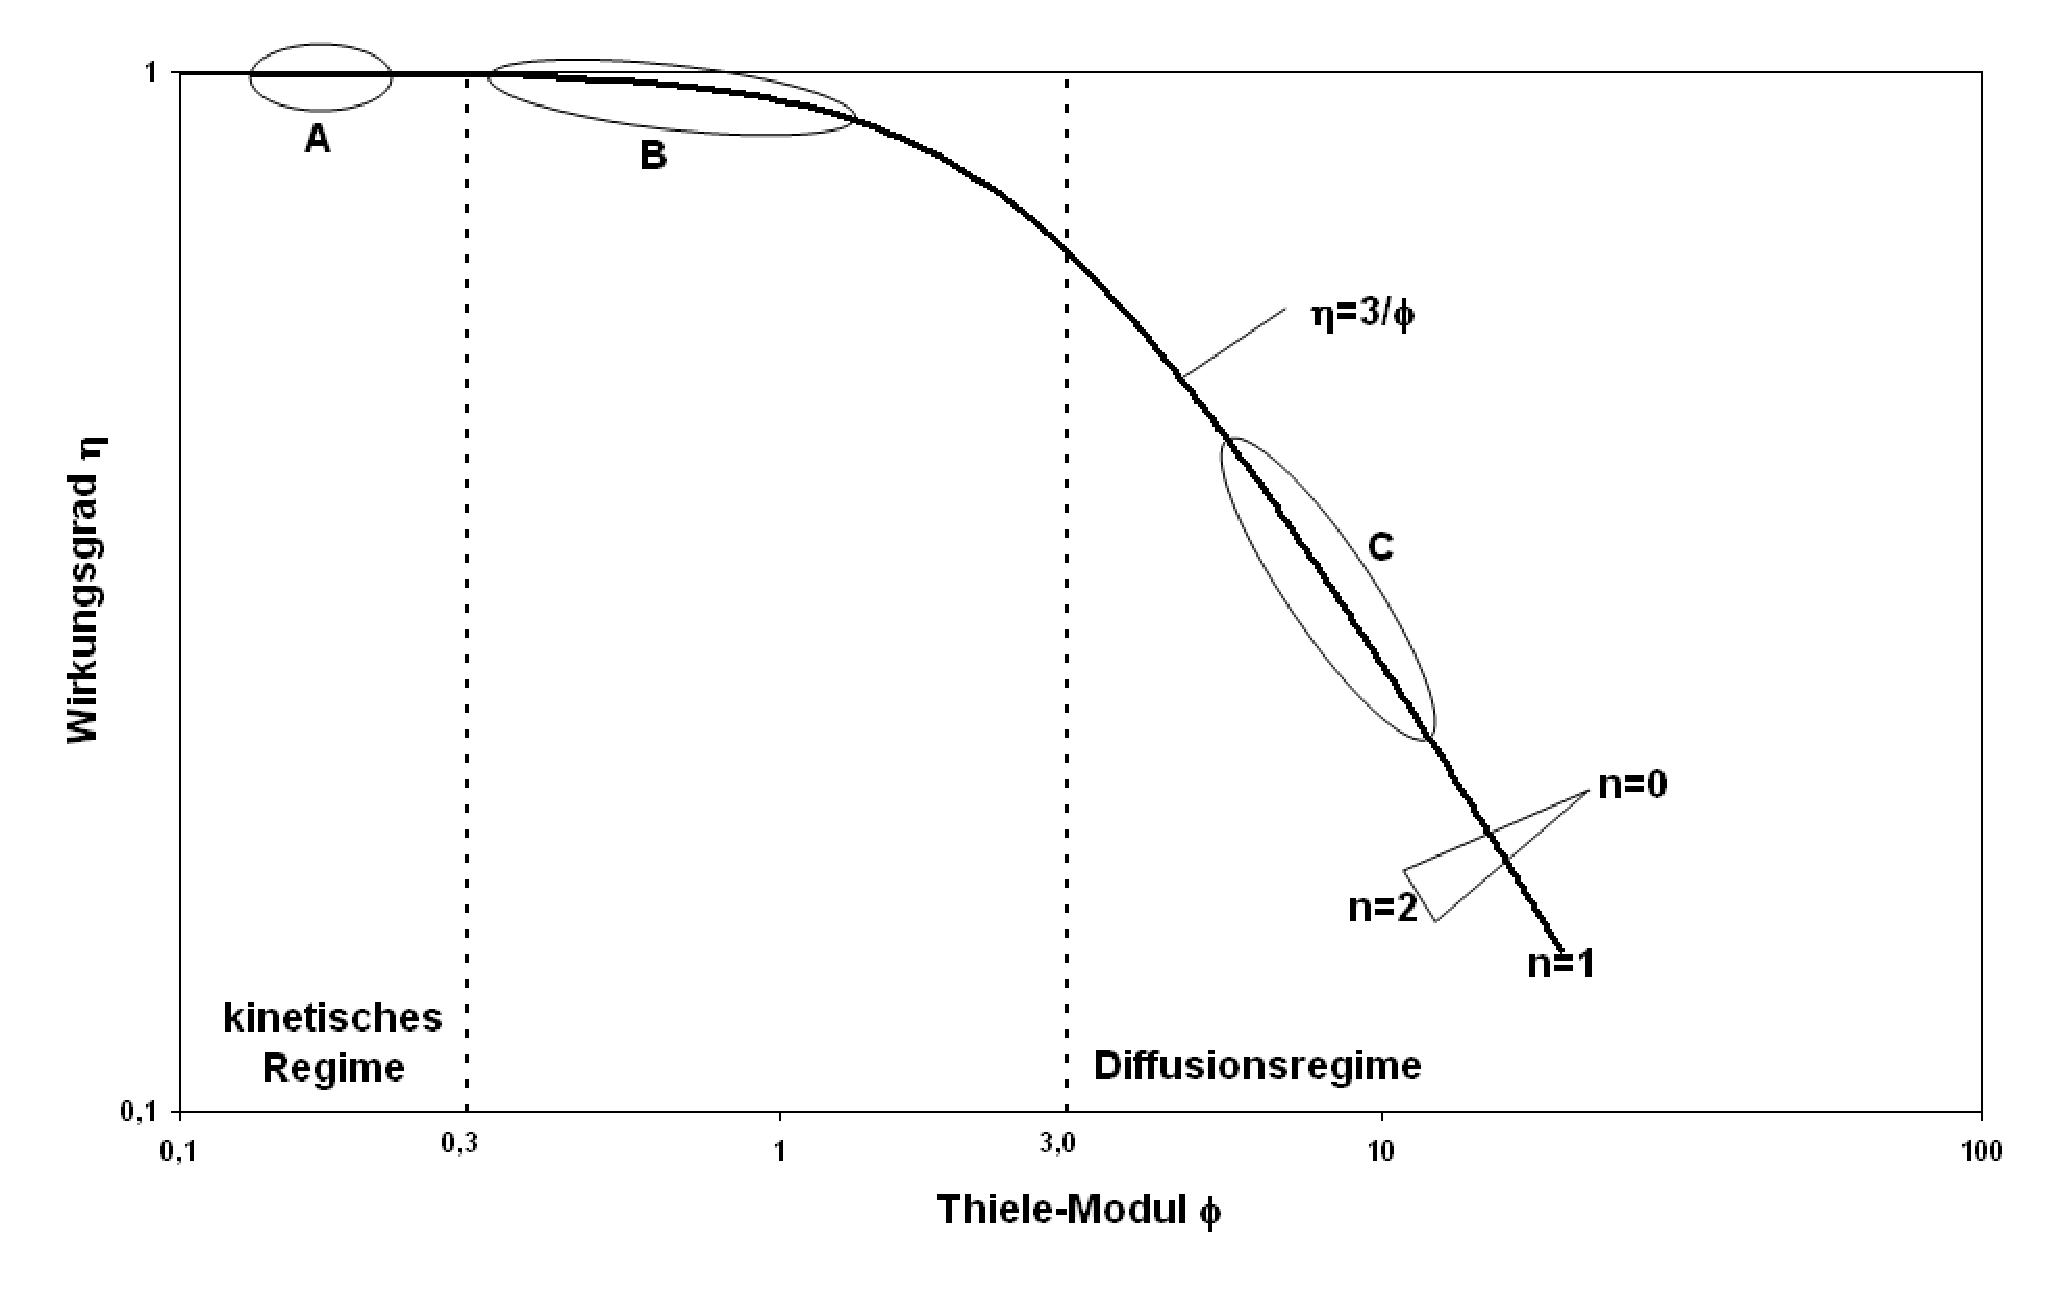
\includegraphics[width=87mm]{images/eta-thiele.eps}
\end{center}
\end{figure}
Mit steigender Reaktionsordnung sinkt die Wirkungsgradkurve nach unten.
\begin{itemize}
\item[A:] Kat mit geringer Aktivit�t: gro�er $D_e$, kleiner $R$ (gro�er Wirkungsgrad, aber hoher Druckverlsut)
\item[B:] angestrebter Betriebszustand: hoher Wirkungsgrad bei gro�em $\Phi$
\item[C:] Kat mit hoher Aktivit�t: niedriger $D_e$, gro�er $R$ (Diffusion hemmt Reaktionsgeschwindigkeit)
\end{itemize}
Je gr��er das {\sc Thiele}-Modul, desto steiler f�llt das Konzentrationsprofil zum Pelletmittelpunkt hin ab.
Bei starker Diffusionshemmung findet die Reaktion deahalb nur in der Randzone statt. Deswegen
schnellere Desaktivierung, da Katalysator unvollst�ndig genutzt.

\subsection{Einfluss der Partikelgr��e}
\begin{figure}[H]
\begin{center}
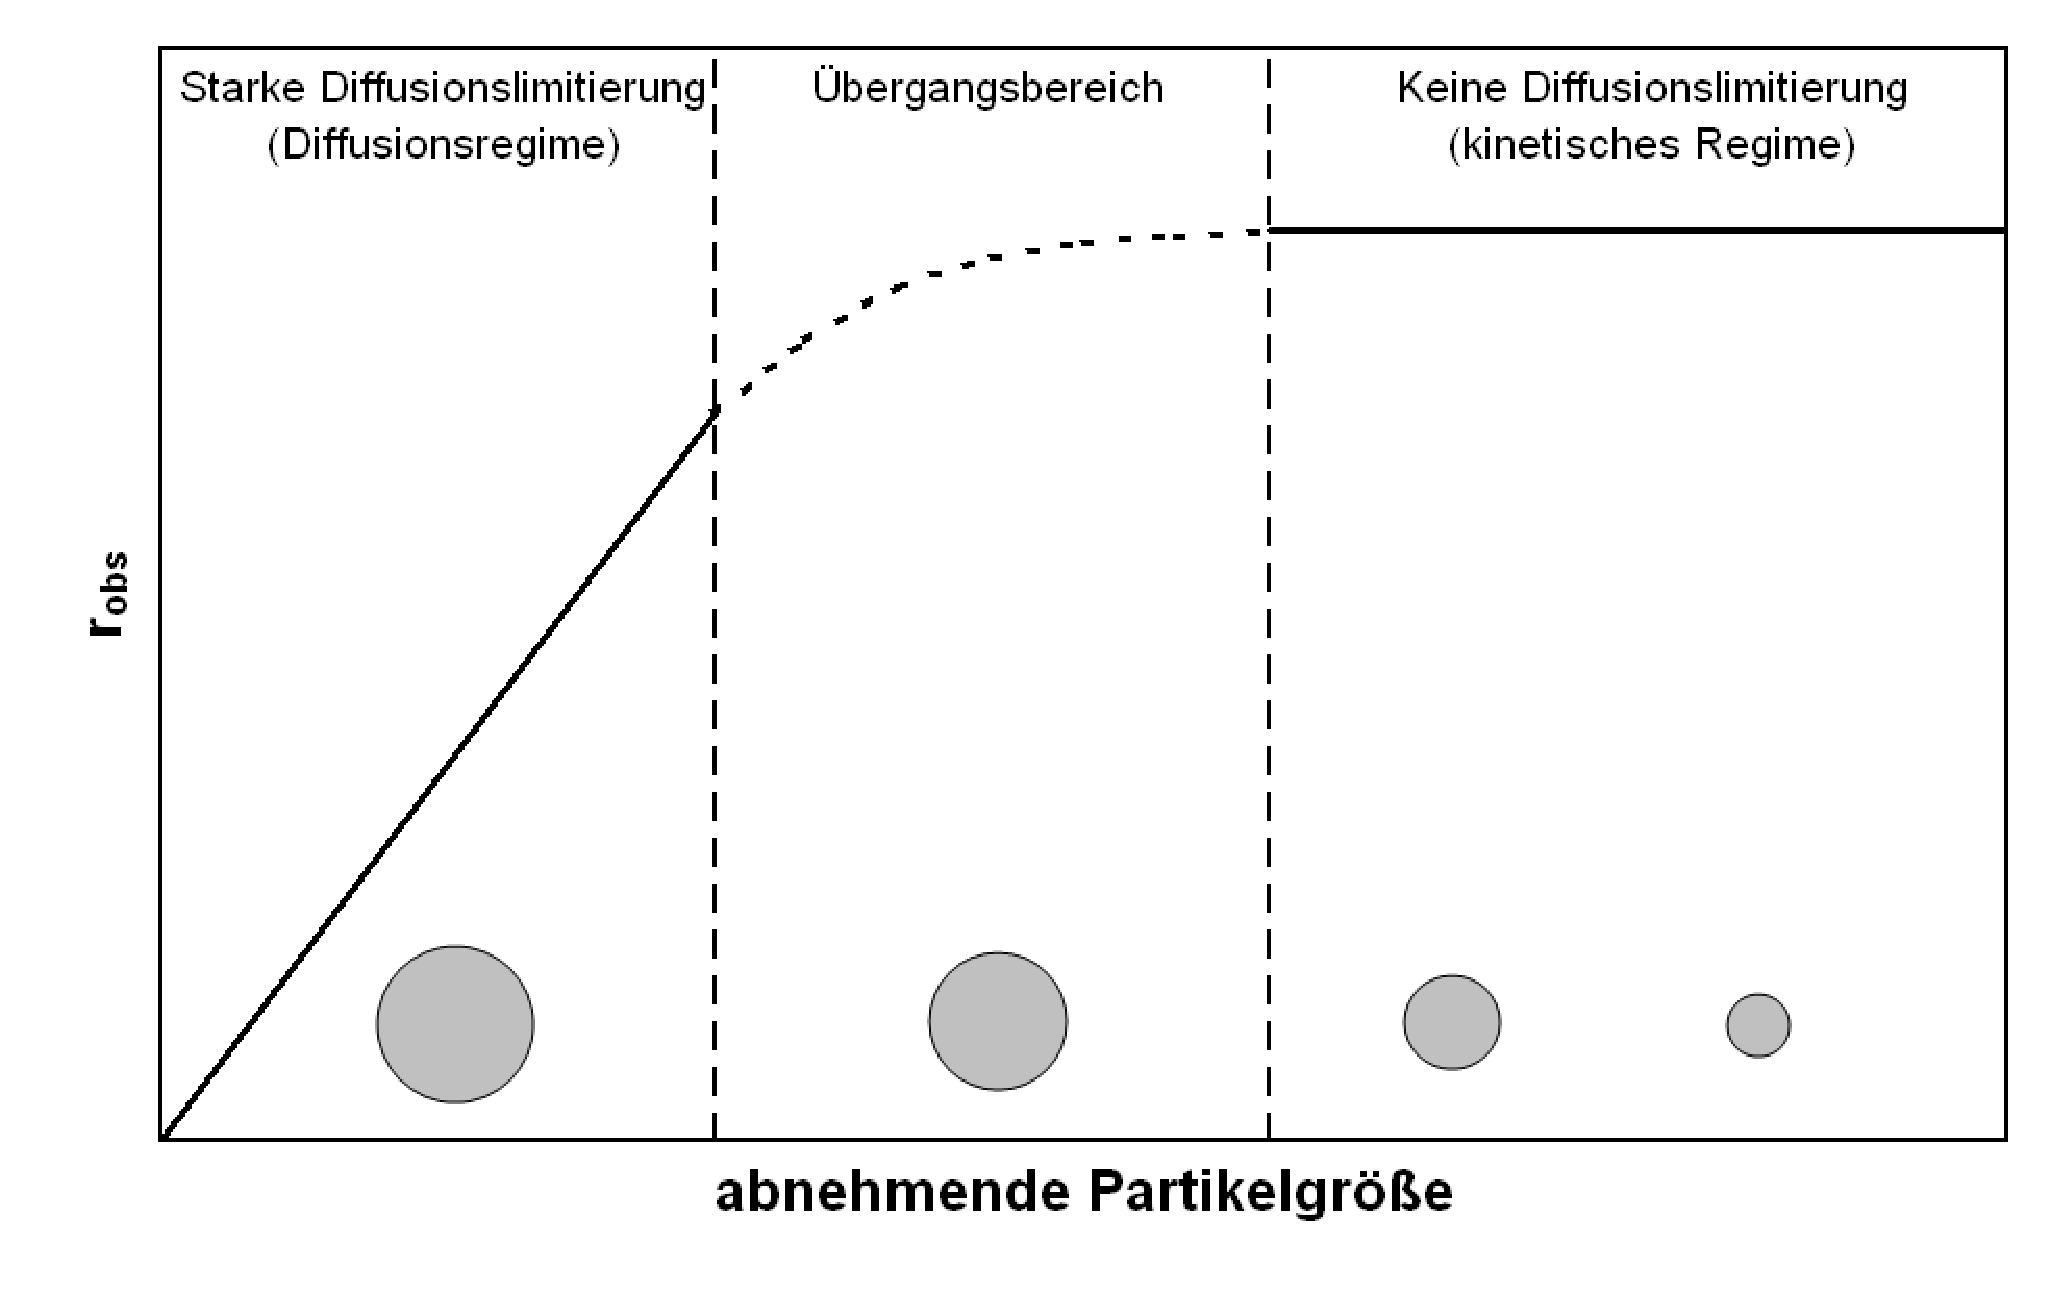
\includegraphics[width=87mm]{images/r_obs-d_p.eps}
\end{center}
\end{figure}

\subsection{Einfluss der Filmdiffusion auf die heterogene Katalyse}
Fluid mit Geschwindigkeit $u$, Dichte $\rho$ und Viskosit�t $\nu$ umstr�mt Katalysatorkorn.\\
Molekulare Diffusion durch die laminare Grenzschicht mit der Filmdicke:
\[ \delta=f\left(u,\rho,\nu,d_p\right) \]
Filmtheorie (1. {\sc Fick}'sches Gesetz):\\
\[ \fbox{$ \displaystyle J=-D\frac{dc}{dx}=\underbrace{\frac{D}{\delta}}_{\beta}\cdot\left(c_b-c_s\right)$} \]
$\beta=f\left(u,\rho,\nu,d_p,D\right)$: Massentransportkoeffizient $\left[\frac{m}{s}\right]$\\
\[ \fbox{$ \displaystyle r_{obs}=\beta\cdot\left(c_b-c_s\right)=k_s\cdot c^n_s = \frac{n_{true}+1}{2} $} \qquad\left[\frac{mol}{m^2s}\right] \]
\begin{table}[H]
\begin{tabular}{p{4.3cm}p{4.3cm}}
\bf Starke Limitierung durch Filmdiffusion	& \bf Keine Limitierung durch Filmdiffusion	\\
(Diffusionsregime)				& (kinetisches Regime)				\\
$\rightarrow$ steiler Konzentrationsgradient	& $\rightarrow$ kein Konzentrationsgradient	\\
$k_s\gg\beta$					& $\beta\gg k_s$				\\	
$r_{obs}=\beta\cdot c_b$			& $r_{obs}=k\cdot c^{n_{true}}_b$		\\
$n_{obs}=1$					& $n_{obs}=n_{true}$				\\
$E_{A,obs}<5\,kJ/mol$				& $E_{A,obs}=E_{A,true}$			\\
\end{tabular}
\end{table}

\subsection{Zusammenwirken von internem und externen Massentransport}
\begin{figure}[H]
\begin{center}
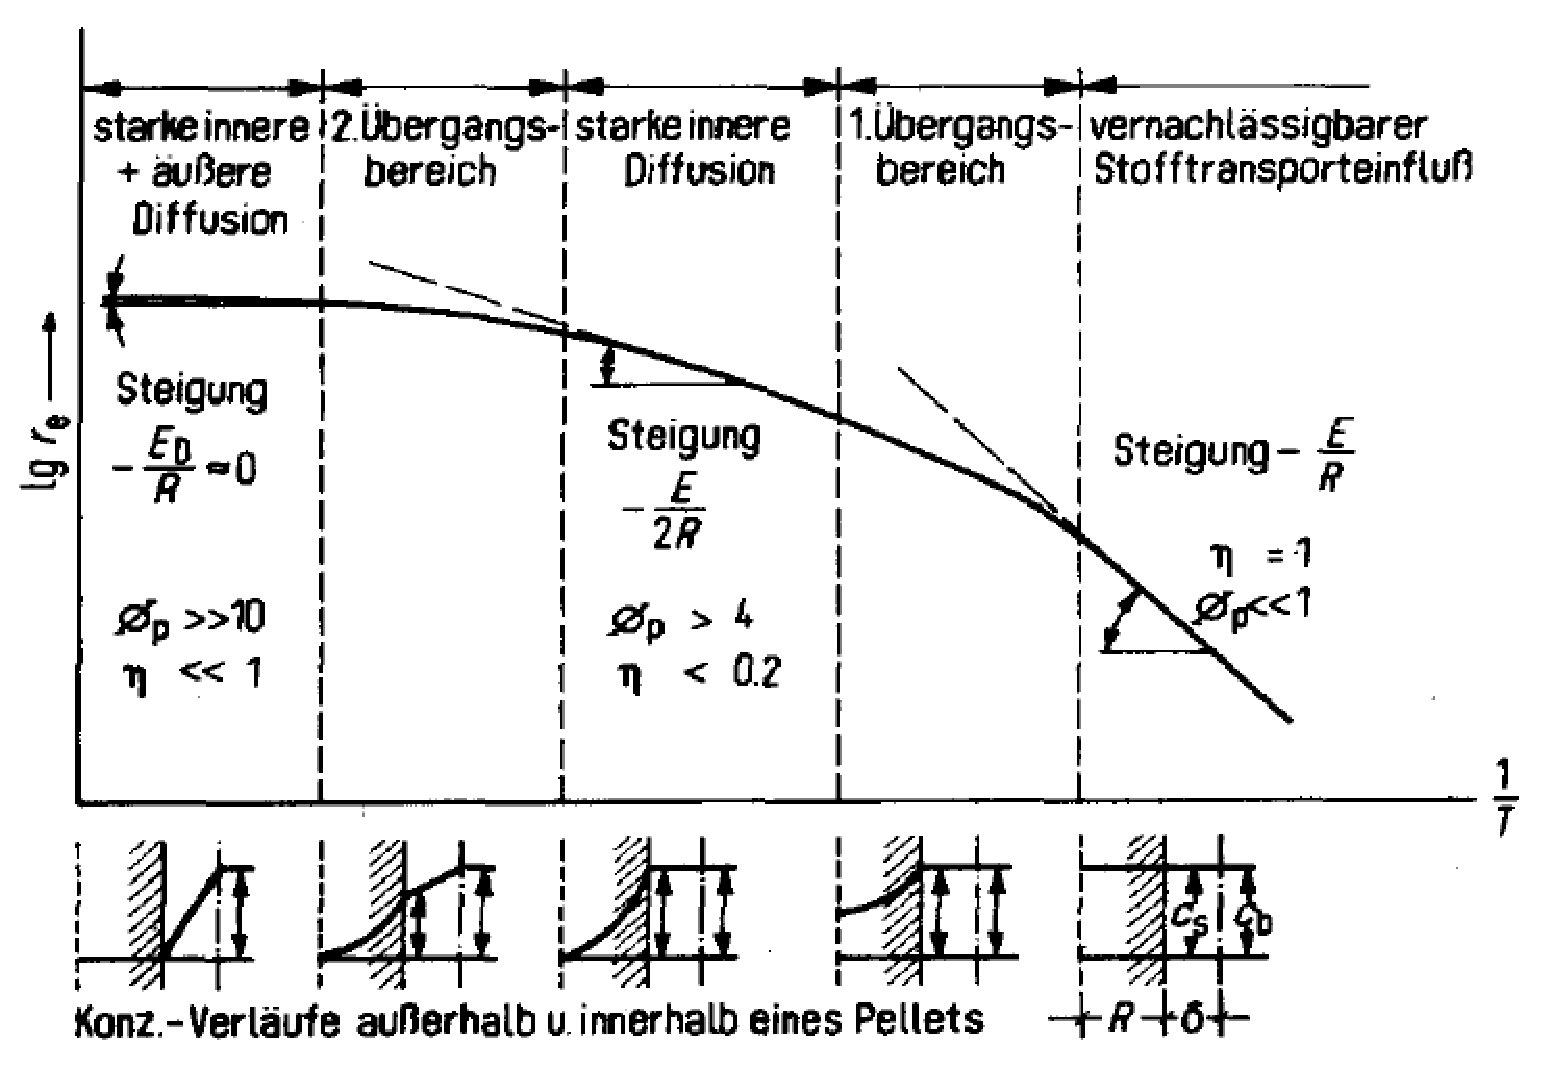
\includegraphics[width=87mm]{images/int-ext.eps}
\end{center}
\end{figure}
Bei sehr hohen Temperaturen:
\begin{itemize}
\item Filmdiffusion (externe Diffusion) kontrolliert den gesamten Prozess.
\item Konzentrationsabfall schon in der �u�eren Grenzschicht.
\end{itemize}
{\sc Biot}-Zahl:\\
\[ \fbox{$ \displaystyle Bi_m=\frac{\beta\cdot R}{D_e}=\frac{\mbox{Massentransport}}{\mbox{Porendiffusion}}$} \]
f�r $Bi_m\rightarrow\infty:\rightarrow c_b=c_s$\\
f�r $Bi_m>100\rightarrow$ Filmdiffusion ist vernachl�ssigbar\\
�bliche Gr��enordnung: $Bi_m=100...200$\\
\[ \eta=f\underbrace{\left(Bi\right.}_{Filmdiffusion};\,\underbrace{\left.\Phi\right)}_{Porendiffusion} \]

\subsection{Gleichzeitiger interner und externer W�rme- und Stofftransport}
{\sc Prater}-Zahl:
\[ \fbox{$ \displaystyle \beta_{Pr}=\frac{c_b\cdot D_e\cdot\left(-\Delta H_R\right)}{\lambda_e\cdot T_b}=\frac{\mbox{max. $\Delta T$ im Pellet}}{\mbox{Bulk-Temperatur}}=\frac{\Delta T_{max}}{T_b}$} \]
Die {\sc Prater}-Zahl quantifiziert das Termperaturgef�lle.
\begin{itemize}
\item $\beta_{Pr}>0$: exotherme Reaktion mit $\eta>1$ (wenn {\it stark} exotherm, selten) und $\eta<1$
\item $\beta_{Pr}<0$: endotherme Reaktion mit $\eta<1$
\end{itemize}
Die {\sc Arrhenius}-Zahl beschreibt den Einfluss der Temperatur auf die Reaktion:\\
\[ \fbox{$ \displaystyle \gamma=\frac{E_A}{RT_b}$} \]

Keine Transporthemmung (willk�rliche Festlegung):
\[\eta=\frac{r_{obs}}{r\left(T_b,\,c_b\right)}=1\pm 0,05 \]
{\sc Weisz-Prater}-Kriterium:\\
\[ \fbox{$ \displaystyle \Phi=\frac{r_{obs}\cdot R^2}{c_s\cdot D_e}=\phi^2\cdot\eta$} \]
$\Phi$: {\sc Weisz}-Modul\\
Keine Limitierung durch Porendiffusion, wenn:\\
$\Phi<6$: Reaktion 0. Ordnung\\
$\Phi<1$: Reaktion 1. Ordnung\\
$\Phi<0,3$: Reaktion 2. Ordnung\\

{\sc Weisz-Hicks}-Kriterium:\\
$\rightarrow$ Pellet nicht isotherem, ausschlie�lich Porendiffusion\\
Keine Massen- und W�rmelimitierung falls 
\[ \Phi\cdot \exp{\left(\frac{\gamma\cdot\beta_{Pr}}{1+\beta_{Pr}}\right)}<1 \]

\subsection{Zweifilm-Theorie}
\subsubsection{Basis}
\begin{itemize}
\item Stagnierende Filme
\item Konzentrationsgradienten
\item Gleichgewicht an Phasengrenzfl�che ($\mu^G = \mu^L$)
\item Diffusion bewirkt Transport durch Grenzfl�che
\end{itemize}

\[ \fbox{$ \displaystyle J_{i,g} = - D_{i,g} \frac{\Delta c_{i,g}}{\delta_g} = J_{i,l} = - D_{i,l} \frac{\Delta c_{i,l}}{\delta_l} $} \]
Treibende Kraft: Chemisches Potential bzw. $\Delta c_i = c_i^* - c_i$!

Stoff�bergangskoeffizienten:
\[ K = \frac{D_i,P}{\delta_P} \]

{\sc Henry} Gesetz (verd�nnte L�sung Gas in Fl�ssigkeit:
\[ p_i^* = H_i c_i^* \]

{\sc Nernst}'sches Gesetz (Liquid/Liquid)
\[ c_{i,I}^* = K_{N} c_{i,II}^* \]

\subsubsection{Bilanz}
Acc = In - Out + React\\
station�r: Acc = 0 \\
\[ (J_1 a)_{y} + (J_1 a)_{y +dy} = k' c_1 c_2 a dy \]
\[ J_1 = -D_{1,l} \left.\frac{dc}{dy}\right|_{y} \qquad \left. \frac{dc_1}{dy} \right|_{y+dy} = \frac{dc_1}{dy} + \frac{dc^2}{dy}dy \]
\[ \rightarrow D_{1,l} \frac{d^2c_1}{dy^2} = k c_1 c_2 \qquad D_{2,l} = \frac{d^2c_2}{dy^2} = k c_1 c_2 \]
Vereinfachungen:
\[ p_1^* = p_{1,g} \qquad c_1^* = \frac{p_{1,g}}{H_1} \qquad k = k' c_2 \]
\[ y = 0: \qquad c_1=c_1^* \qquad c_2=c_{2,l} \]
\[ y = \delta_l: \qquad c_1 = c_{1,l} \qquad c_2 = c_{2,l} \]
\[ \fbox{$ \displaystyle d_{1,l} \frac{d^2c_2}{dy^2} = k c_1 $} \]

Mit Hilfe der dimensionslosen {\sc Hatta}-Zahl:
\[ \fbox{$\displaystyle Ha = \delta \sqrt{\frac{k c_1^{* n-1}}{D_{1,l}}} $} \]
Das analoge {\sc Thiele}-Modul stellt das Verh�ltnis von Reaktion zu Diffusion bei Fluid-Fest (Katalysator) Reaktionen dar, w�hrend die
{\sc Hatta}-Zahl selbiges f�r Fluid-Fluid Reaktionen quantifiziert.

\[ Ha = \delta_l \sqrt{\frac{k}{D_{1,l}}} = \frac{\delta_l}{D_{1,l}} \sqrt{k D_{1,l}} = \frac{1}{k_{1,l}} \sqrt{k D_{1,l}} \]

\subsubsection{Chemische Reaktion und Stofftransport}
\begin{enumerate}
\item Chemische Reaktion im Bulk
\item Stofftransport durch Fl�ssigkeitsfilm ist langsamer als Reaktion $\rightarrow$ Reaktion im Film
\end{enumerate}


\section{Auswertung kinetischer Daten}
\subsection{Scale-Up}
Problem beim Scale-Up von der Laboranlage zur gro�technischen Anlage sind:
\begin{itemize}
\item Form des Reaktors
\item W�rmezu- und abfuhr
\item Str�mungsbedingungen
\item Vermischungsverhalten
\end{itemize}
Als Methoden f�r den Scale-Up ergeben sich:
\begin{table}[H]
\begin{tabular}{c|c} 
\bf klassisch	& \bf modern \\ \hline
emprische Betrachtung & Detailverst�ndnis + Modellbildung \\
stufenweiser Scale-Up & in einem Schritt \\
kostenintensiv & interdisziplin�r \\
Grundoperationen & Prozessdenken \\
\end{tabular}
\end{table}

\subsection{Ziel kinetischer Messungen}
Mikrokinetik
\begin{itemize}
\item nicht Transportlimitiert
\item Beschreibung durch intrinsische Kinetik oder Kenntnis des Mechanismus
\item formalkinetisch vereinfachende Annahmen
\end{itemize}
Makrokinetik
\begin{itemize}
\item Effektivkinetik mit Transporteinfluss
\item nicht getrennt von Transport
\item Beschreibung durch Scale-down 
\end{itemize}

\subsection{Prinzipien von Betriebsweise und Bauart}
Ist der Reaktor
\begin{itemize}
\item komplex oder einfach?
\item isotherm, adiabat oder polytrop?
\item Homogen oder Heterogen?
\end{itemize}
L�sung: Bestimmung von Konzentrationen in Abh�ngigkeit von der Zeit ($c= f(\tau)$ bzw $c = f(t_R)$)!\\
BSTR: Zeitkonstante = $t_R$\\
PFTR: Zeitkonstante = $\tau$

\subsubsection{Differentialreaktoren}
Bei Differentialreaktoren kann bei kleinen Ums�tzen die Reaktionsgeschwindigkeit direkt bestimmt werden:
\[ \nu_{i} r = \frac{c_{i0}-(c_{i0}-dc_i)}{dt} = - c_{i0} \frac{dX_i}{dt} \]
In der Praxis ist allerdings $\frac{dX_i}{dt}$ schwer bestimmbar. Damit ist das Ergebnis einem $T$ bzw. $c$ nicht mehr genau zuzuordnen!

\subsubsection{Schlaufenreaktor}
Ein idealer CSTR verh�lt sich wie ein Schlaufenreaktor - Also gro�er Recycle Strom, gradientenlos.\\
Die Stoffmengen�nderungsgeschwindigkeit ergibt sich zu:
\[ R_i = - \frac{\dot{n}_{i0} - \dot{n}_i}{V} \qquad R_k = \frac{\dot{n}_{k0}dX_k}{m_{cat}} \]

\subsection{Beispiele f�r spezielle Rohrreaktoren}
\subsubsection{Heterogen Katalysierte Reaktionen}
Hier w�hlt man meist
\begin{itemize}
\item Rohrreaktor mit F�llung $\rightarrow$ Festbettreaktor
\item Schlaufenreaktor mit innerem und �u�erem Kreislauf
\end{itemize}
\[ r = \frac{1}{\nu_i} \frac{dn}{dt} \frac{1}{m_{kat}} \]

\subsubsection{Fluid-Fluid-Reaktoren}
Hier ist der Stofftransport von sehr gro�er Bedeutung!
\begin{itemize}
\item Mikrokinetik oder Transportlimitierung bestimmen
\item Bestimmung der Makrokinetik in Reaktor mit bekannter Fluiddynamik und Austauschfl�che
\end{itemize}
\begin{enumerate}
\item Laminarer Fallfilmabsorber\\
Es werden Eingangs- und Ausgangskonzentrationen gemessen. Sehr interessant, wegen definierter Verweilzeit und Phasengrenzfl�che.\\
Besonders gut geeignet bei schnellen Reaktionen (sehr gro�e Ha-Zahl!)
\item Laminarstrahlabsorber \\
Durch die wechselnden Str�mungsprofile ist die Verweilzeit berechenbar durch
\[ \tau = \frac{\pi d^2 L}{4 \dot{V}_l} \]
\end{enumerate}

\subsection{Methoden der Auswertung}
Aufstellen eines Modell, wobei dessen Parameter bestimmt werden m�ssen.
\begin{enumerate}
\item Kinetische Modellrechnung
\[ \begin{array}{r} r \\ X \\ ... \end{array} = f\left( \begin{array}{l} c_i \\ p_i \\ T \\ m_{cat} \\ ... \end{array} \right) \]
\item Parameterabsch�tzung
\item Struktur des Reaktionsschemas ermitteln (bei komplexen Reaktionen)
\end{enumerate}
In der Vergangenheit dominierten eher graphische Methoden, heute sind es eher statistische.

\subsection{Differentialmethode}
Reaktionsrate wird aus $c-t$-Plot mit Hilfe graphischer oder numerischer Differentiation ermittelt.
Vorteil ist die generelle Anwendbarkeit und der geringe Aufwand der Berechnung.  Demgegen�ber steht der Nachteil, dass die Reaktionsrate sehr schwer messbar ist und dass die Differentation prinzipbedingt einen gewissen Fehler aufweist.

\subsubsection{bei Potenzans�tzen}
\[ \fbox{$ \displaystyle r = k c_i^m $} \quad \rightarrow \quad \fbox{$ \displaystyle \ln r = \ln k + m \ln c_i $}\]
Graphische Auftragung $\ln r$-$\ln c_i$. Achsenabschnitt: $\ln k$, Steigung $m$.

\subsubsection{bei hyperbolischen Ans�tzen}
\[ \fbox{$ \displaystyle r = \frac{k p_i}{1 + K p_i} $} \quad \rightarrow \quad r + K p_i r = k p_i \]
\[ \fbox{$ \displaystyle \frac{p_i}{r} = \frac{K}{k} p_i + \frac{1}{k} $} \]
Graphische Auftragung $\frac{p_i}{r}$-$p_i$. Achsenabschnitt: $\frac{1}{k}$, Steigung: $\frac{K}{k}$.

\subsection{Integralmethode}
\[ \fbox{$ \displaystyle \frac{dc}{dt} = - k c^m $}\quad \rightarrow \quad \begin{array}{l@{\quad}r@{\,=\,}l} m = 1 & \ln c - \ln c_0 & -kt \\ m \ne 1 & \frac{1}{c^{m-1}}-\frac{1}{c_0^{m-1}} & (m-1) kt \end{array} \]
Wichtig hierbei: Parameter $m$ wird angepasst, bis sich eine Gerade ergibt!

\section{Typen von Reaktionsapparaten}
\subsection{Nach Art der Betriebsweise}
\subsubsection{Diskontinuierlicher Batch-Reaktor}
Zusammensetzung der Komponenten im Apparat �ndern sich st�ndig. Reaktor arbeitet insation�r f�r eine definierte Zeit.\\
Vorteile:
\begin{itemize}
\item Flexibilit�t
\item hohe Ums�tze durch beliebig lange Reakionszeiten
\end{itemize}
Nachteile:
\begin{itemize}
\item Totzeiten durch F�llen, Entleeren, S�ubern
\item hoher Steuer und Regelungsaufwand
\end{itemize}
Anwendungen sind somit die Specialties mit $< 1000t/a$.

\subsubsection{Kontinuierliche Betriebsweise}
Edukte werden kontinuierlich zugef�hrt, Produkte kontinuierlich abgezogen. Alle Prozessparamter sind konstant. Reaktor arbeitet somit statinon�r.
Vorteile:
\begin{itemize}
\item Gut Automatisierbar
\item Geringe Stillstandszeiten
\item gleichbleibende Produktqualit�t
\end{itemize}
Nachteile:
\begin{itemize}
\item geringere Flexibilit�t
\item Eduktqualit�t muss gleichbleibend sein
\item hohe Investitionskosten
\end{itemize}
Anwendung sind Gro�produktionen. Allerdings werden zunehmen auch kontinuierliche Mikroreaktoren an Stelle von Batchreaktoren eingesetzt.

\subsubsection{Halbkontinuierliche Prozesse}
\begin{enumerate}
\item Ein Reaktand liegt im �berschuss zu, der andere wird sukzessive zugegeben.\\
Bsp. Nitrierung von Benzol
\item Ein Produkt wird kontinuierlich abgezogen, zwecks Verschiebung des Gleichgewichts.\\
Bsp. Abziehen von Wasser bei der Veresterung
\item Ein Reaktand liegt vor, anderer wird zugegeben, Produkt wird kontinuierlich abgezogen.
\end{enumerate}

\subsection{nach Art der Phasen}
\subsubsection{Einphasige Systeme}
\paragraph{R�hrkessel}
\begin{itemize}
\item sowohl Batch/Fed-Batch oder Konti einsetzbar
\item Dampf/K�hlwasser f�r W�rmetausch durch Heiz- oder K�hlschlangen
\item Verschiedene Reaktoren mit unterschiedlichen Leistungs- und Mischzeitcharakteristika
\end{itemize}

Wichtig hier, ist besonders die Auswahl des geeigneten Misch bzw. R�hrger�tes. Hierbei ist das wichtigste Auswahlkriterium die Viskosit�t.
Zus�tzlich ist noch nach der gew�nschten vorherrschenden Str�mungsrichtung (radial oder axial) auszuw�hlen.\\
Kriterium f�r die Eignung eines R�hrers ist:
\begin{itemize}
\item Batch-Reaktor: Mischzeit sollte kleiner als die Zeitkonstante der Reaktion sein: \[ t_m \le 0,1 \frac{c_{1,0}}{r_0} \]
\item Konti-Reaktor: Mischzeit sollte kleiner als die hydrodyn. Verweilzeit sein: \[ t_m \le 0,1 \tau \]
\end{itemize}

\paragraph{Str�mungsrohre}
Analogie: Str�mungsrohr $\leftrightarrow$ diskont. R�hrkessel! Vergleiche $c_{PFTR}$-$\tau \quad$ und $\quad c_{BSTR}$-$t_R$, diese sind identisch!\\
Str�mungsrohre eignen sich vor allem bei
\begin{itemize}
\item stark exo-/endothermen Reaktionen, da W�rmeaustauschfl�che bezogen auf Volumen sehr gro� ist
\item Reaktionen mit hohem Durchsatz
\end{itemize}
Einsatzbeispiel: Streamcracking

\subsubsection{Mehrphasige Systeme}
In mehrphasigen Systemen spielen W�rme- und Stofftransport eine entscheidende Rolle f�r Umsatz und Selektivit�t.
Entscheidende Entscheidende Parameter hierbei sind vor allem: Stoff- / W�rme�bergangskoeffizienten und die Austauschfl�che.
\paragraph{Fluid-Feststoff}
Reaktion an Oberfl�che mit Verbrauch des Feststoffes oder Katalyse.\\
Festbettreaktoren k�nnen isotherm, polytrop oder adiabat betrieben werden.\\
Zur Begrenzung der Temperatur bieten sich an:
\begin{itemize}
\item Rohrb�ndelreaktor (Multitubular Reactor)
\item Hordenreaktor (Rack-type Reactor)
\end{itemize}
\paragraph{Wirbelschichtreaktoren}
Vorteile von Wirbelschichtreaktoren sind
\begin{itemize}
\item Feststoff ist im fluidisierten Zustand einfach zu handlen
\item Nutzung sehr kleiner Partikel leicht m�glich. Dadurch geringe Makrokinetische Limitierung
\item Gute radiale und axiale Vermischung
\item Guter W�rme�bergang
\end{itemize}
Nachteile
\begin{itemize}
\item Breite Verweilzeitverteilung
\item Abrasive Effekte
\item Modellierung schwierig
\end{itemize}
F�r Details zu Wirbekschichten: MVT Scriptum!
Hier nur kurz:
\[ \Delta p S = (1 -\varepsilon_{mf})SHg(\rho_p-\rho_g) \]

\paragraph{Fluid-Fluid-Systeme}
\begin{enumerate}
\item Gas dispergiert in Fl�ssigkeit\\
  Blasens�ule, Bodenkolonne, R�hrkessel
\item Fl�ssigkeit in Gas dispergiert\\
  Strahlw�scher, Spr�hturm
\item Fl�ssigkeit wird dem Gas als d�nner Film ausgesetzt\\
  Fallfilmreaktor, Trickle-Bed-Reaktor
\end{enumerate}
Zur Beurteilung der einzelnen Varianten bietet sich die Kennzahl B an.
\[ \fbox{$ \displaystyle B = \frac{A\rho}{V_l} $} \]
In Abh�ngigkeit der Ha-Zahl ergibt sich im Graph gegen $\eta$ folgendes Bild:
\begin{figure}[H]
\beginpicture
\setcoordinatesystem units <2cm,2cm>
\setplotarea x from -4 to 0, y from -2 to 0
\axis bottom label {$\log B$} ticks numbered from -4 to 0 by 1 unlabeled short from -4 to 0 by 0.1 /
\axis left label {\rotatebox{90}{$\log \eta$}} ticks numbered from -2 to 0 by 1 unlabeled short from -2 to 0 by 0.1  /
\axis top /
\axis right /
\linethickness 0.1pt
\setdots <2pt>
\linethickness 1pt
\setquadratic
\setsolid
\plot -4 -0.3 -3 -0.06 0 0 /
\plot -4 -1.3 -2.65 -0.3 0 0 /
\plot -4 -2 -2.5 -0.5 0 0 /
\plot -3 -2 -1.8 -0.7 0 0 /
\plot -2.1 -2 -1 -0.8 0 -0.15 /
\setlinear
\plot -1.5 -2 0 -0.5 /
\put {Ha = 0,01} at -3.5 -0.35
\put {0,05} at -3.75 -0.7
\put {0,1} at -3.2 -0.7
\put {0,3} at -2 -0.7
\put {1,0} at -1.15 -0.7
\put {3,0} at -0.2 -1
\endpicture
\end{figure}
�bliches Einsatzgebiet ist: $2\cdot10^{-4} < B < 10^{-1}$.\\
\begin{itemize}
\item F�r kleine Ha-Zahlen sorgt ein gr��eres B (Oberfl�che!) nicht f�r gr��ere Kapazit�ten (Reaktion im Bulk!)
\item F�r schnelle Reaktionen (gro�e Ha) muss eine gro�e Oberfl�che (B!) bereitgesetllt werden, da sonst $\eta$ sehr klein wird.
\end{itemize}

\paragraph{Dreiphasige Systeme}
Hier treten Gas, Fl�ssigkeit und Feststoff in Wechselwirkung.
\begin{itemize}
\item Blasens�ule mit Packung
\item Rieselbettreaktor
\item Dreiphasige Wirbelschicht
\item Suspensionsreaktoren
\end{itemize}

\section{Modellierung idealer Reaktoren}
\begin{table}[H]
\begin{tabular}{lcl}
\bf Ideale Reaktoren	& $\leftrightarrow$	& \bf Reale Reaktoren \\
einfachster Fall,	&			& beliebig kompliziert\\
Grenzfall		&			& Kombination von Elementen\\
			&			& idealer Reaktoren\\
\end{tabular}
\end{table}
Zwei Grenzf�lle:
\begin{itemize}
\item ideale Vermischung bis in die molekulare Ebene; z.B. CSTR
\item keine axiale Vermischung; z.B. PFTR
\end{itemize}
\subsection{Systematik des Bilanzierens}
Wir brauchen:
\begin{itemize}
\item Geschwindigkeitsgleichung f�r Reaktion und physikalische Transportprozesse
\item Erhaltungss�tze f�r\\
- Masse (Stoffmenge) $\rightarrow$ Variable $c_i$\\
- Energie (Enthalpie) $\rightarrow$ Variable $T$\\
- Impuls $\rightarrow$ Variable $p$
\end{itemize}
Geeignete Bilanzgrenzen m�ssen definiert werden, z.B.:\\
gesamte Anlage, Reaktor, Fluidelement, Katalysatorpartikel, etc.\\
 
Allgemeine Wortgleichung:\\
$[$Akkumulation$]=[$Zustrom$]-[$Abstrom$]+[$Quelle/Senke$]$\\
Massenbilanz:\\
\[ \fbox{$\displaystyle \underbrace{\frac{\partial c_i}{\partial t}}_{\mbox{Akk.}}=\underbrace{-div \left(c_i\bar u\right)}_{\mbox{Konvektion}}
+\underbrace{div \left(D^e_i grad c_i\right)}_{\mbox{Dispersion}}+\underbrace{\sum_j\nu_{ij}r_j}_{\mbox{Reaktion}}$}\qquad\left[\frac{kmol}{m^3s}\right]  \]
W�rmebilanz:\\
\[ \fbox{$\displaystyle \underbrace{\frac{\partial\left(\rho c_pT\right)}{\partial t}}_{\mbox{Akk.}}=
\underbrace{-div\left(\rho c_p T\bar u\right)}_{\mbox{Konvektion}}+\underbrace{div\left(\lambda^e grad T\right)}_{\mbox{eff. W�rmeltg.}}+
\underbrace{\sum_j\left(-\Delta H_R\right)_jr_j}_{\mbox{Reaktion}}$}\qquad\left[\frac{kJ}{m^3s}\right]  \]
Impulsbilanz:\\
\[ \frac{\partial(\rho u)}{\partial t} + \nabla ( \rho u^2 ) - g \rho = 0 \]

Bedeutung von Differentialoperatoren:\\
\[ \underbrace{div D^e_i\underbrace{grad\underbrace{c_i}_{\mbox{Skalar}}}_{\mbox{Vektor}}}_{\mbox{Skalar}}=\underbrace{D^e_i\left(\frac{\partial^2c_i}{\partial x^2}+ \frac{\partial^2c_i}{\partial y^2}+\frac{\partial^2c_i}{\partial z^2}\right)}_{\mbox{2. {\sc Fick}'sches Gesetz}} \]
Divergenz $div$ transformiert Vektor in Skalar\\
Gradient $grad$ transformiert Skalar in Vektor\\
\subsection{idealer R�hrkessel}
Vollkommene Gleichheit der Konzentrationen und der Temperatur $\rightarrow$ Terme f�r Dispersion und W�rmeleitung entfallen.\\
Massenbilanz:
\[ \fbox{$\displaystyle \underbrace{\frac{dc_i}{dt}}_{\mbox{Akkumulation}}=\underbrace{\frac{\dot V_0}{V}c_{i0}}_{\mbox{Zustrom}}-\underbrace{\frac{\dot V_e}{V}c_{i}}_{\mbox{Abstrom}}+\underbrace{\sum \nu_{ij} r_j}_{\mbox{Reaktion}}$}  \]
W�rmebilanz:
\[ \fbox{$\displaystyle \underbrace{\rho c_p\frac{dT}{dt}}_{\mbox{Akk.}}=
\underbrace{\frac{\dot V_0}{V}\rho c_pT_0}_{\mbox{Zustrom}}-\underbrace{\frac{\dot V_e}{V}\rho c_pT}_{\mbox{Abstrom}}+
\underbrace{\sum_j\left(-\Delta H_R\right)_jr_j}_{\mbox{Reaktion}}-\underbrace{\dot Q(T)}_{\mbox{W�rmezu/-abfuhr}}$} \]
Vereinfachungen:\\
station�rer Zustand: $\frac{dc}{dt}=0$\\
konstantes Volumen: $\dot V=\dot V_e=\dot V_0$\\
\[ \fbox{$\displaystyle c_i-c_{i,0}=\tau\sum_j\nu_{ij}r_j $} \]
Umsatz f�r Reaktion 1. Ordnung:\\
\[ X=\frac{\tau k}{1+\tau k}=\frac{DaI}{1+DaI} \]
\begin{figure}[H]
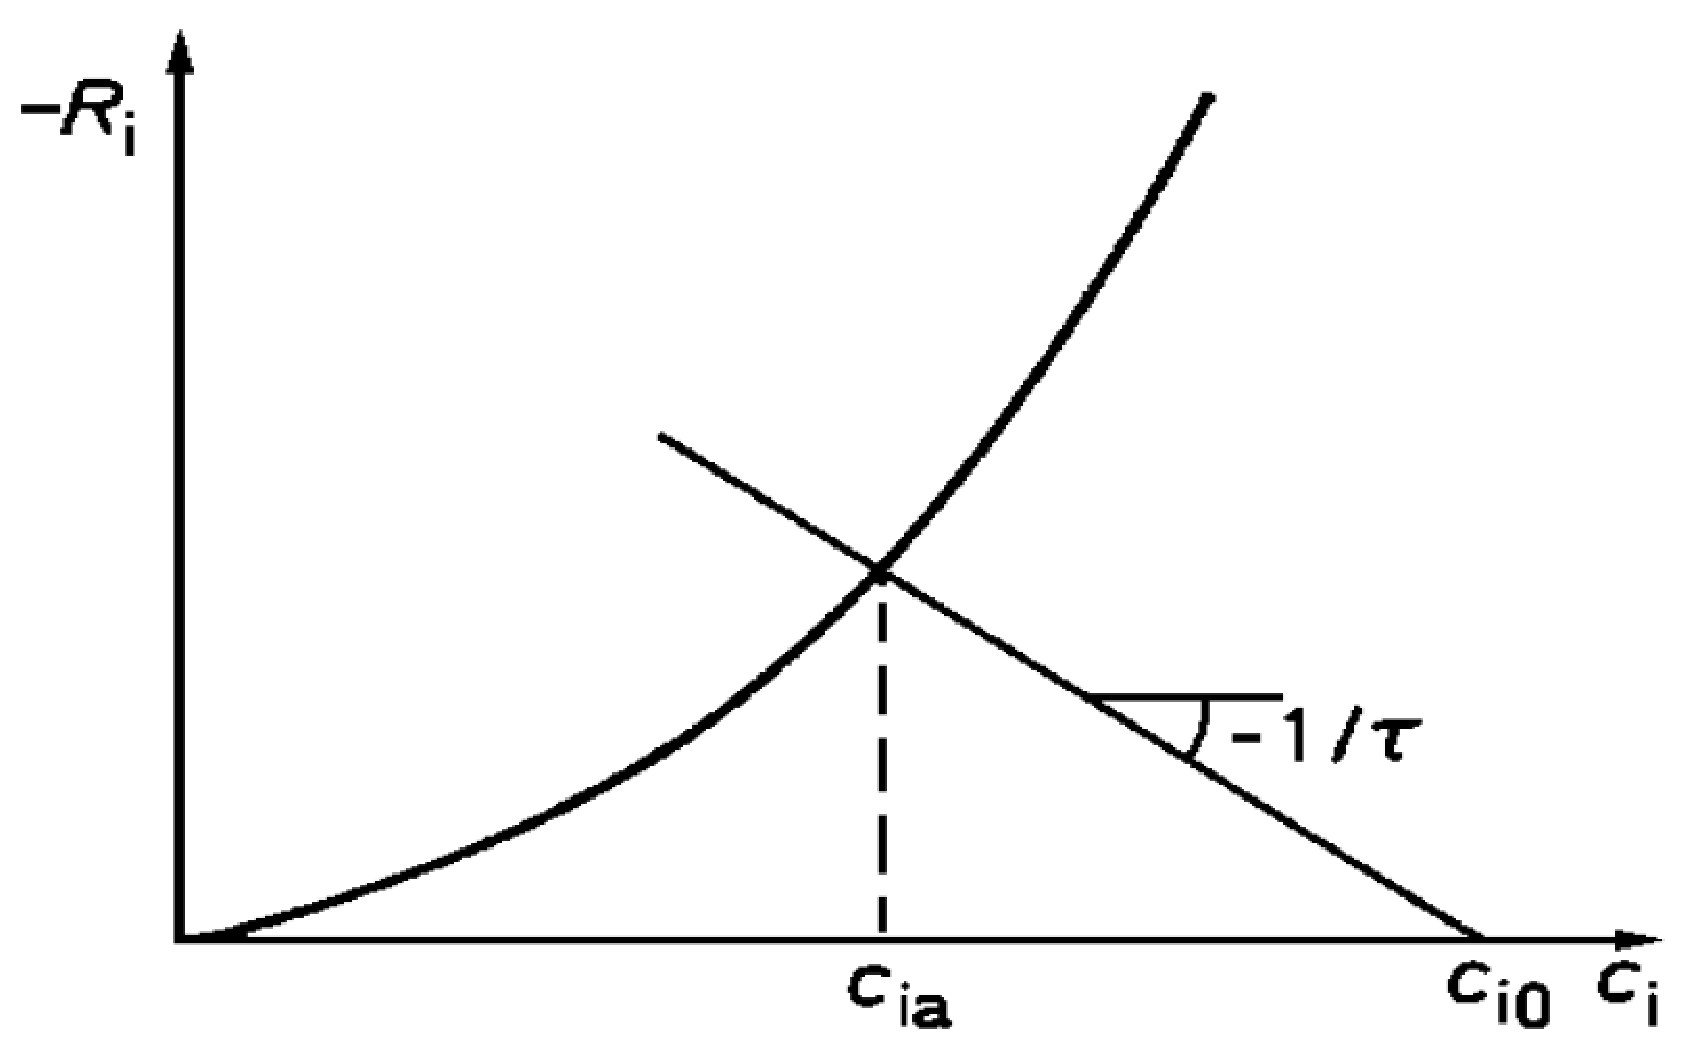
\includegraphics[width=87mm]{images/cstr.eps}
\end{figure}
\subsubsection{R�hrkesselkaskade}
Massenbilanz f�r den k-ten Kessel:
\[ \fbox{$\displaystyle \frac{dc_{i,k}}{dt}=\frac{1}{\tau_k}c_{i,k-1}-\frac{1}{\tau_k}c_i,k+\sum_j\nu_{ij}r_j $} \]
Umsatz der R�hrkesselkaskade kann grafisch �ber Treppenzugverfahren bestimmt werden.\\
Ein PFTR gleicht einer R�hrkesslekaskade mit unendlich vielen Kesseln.\\
Der Umsatz einer R�hrkesselkaskade bleibt immer in den Grenzen zwischen R�hrkessel ($K=1$) und idealem Str�mungsrohr ($K=\infty$).
\begin{figure}[H]
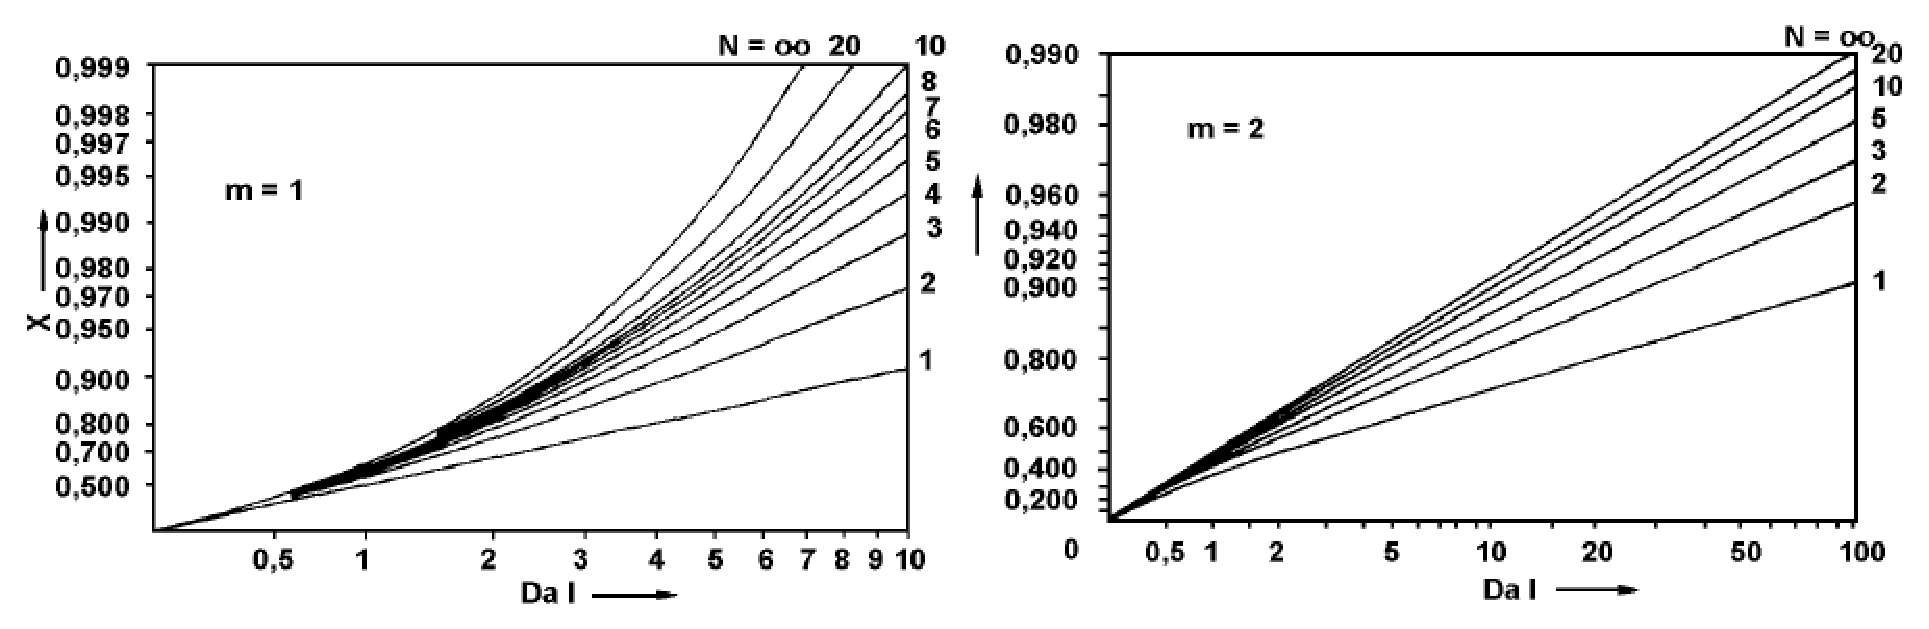
\includegraphics[width=87mm]{images/umsatz.eps}
\end{figure}
\begin{itemize}
\item F�r Reaktionen erster und zweiter Ordnung sind die Ums�tze in Str�mungsrohren immer gr��er als in einem idealen R�hrkessel mit dem selben Volumen.
\item F�r gleiche DaI sind die Ums�tze f�r Reaktionen 1. Ordnung immer gr��er als f�r Reaktionen 2. Ordnung.
\end{itemize}
Gew�hnlich werden in der Technik Kaskaden mit zwei bis f�nf Kesseln realisiert.
Hier liegt das Optimum zwischen h�herem Umsatz und Investitionskosten.  
\subsubsection{Halbkontinuierliche (semi-batch) Betriebsweise}
Ein Reaktand wird im Reaktor vorgelegt, der andere wird kontinuierlich hinzugegeben.\\
Diese Betriebsweise wird f�r stark exotherme Reaktionen, wie z.B. Nitrierungen, verwendet.\\
Stoffmengenbilanz f�r den kontinuierlich zugegebenen Reaktanden $A_1$:\\
$\dot V_e=0$; Reaktionsvolumen $V(t)$ ist zeitabh�ngig
\[ \fbox{$\displaystyle \frac{dn_1}{dt}=\dot V_1c_{i,0}-V(t)\cdot r$} \]
\subsubsection{Diskontinuierliche (batch) Betriebsweise}
Es entfallen die Terme f�r Konvektion und Dispersion.\\
Massenbilanz:\\
\[ \fbox{$\displaystyle \frac{dc_i}{dt}=\sum_j\nu_{ij}r_j$}  \]
W�rmebilanz:\\
\[ \fbox{$\displaystyle \rho c_p\frac{dT}{dt}=\sum_j\left(-\Delta H_R\right)_jr_j-\dot Q(T)$} \]
Bestimmung der Reaktionszeit $t_R$:
\[ \fbox{$\displaystyle t_R=n_{1,0}\int_{X=0}^{X_R}\frac{dX}{rV}$}  \]
Zur grafischen Bestimmung von $t_R$: Auftragung von $\frac{1}{rV}$ gegen $X$.\\
$\rightarrow$ Integral von $0$ bis $X_R$ entspricht $\frac{t_R}{n_{1,0}}$.
\begin{figure}[H]
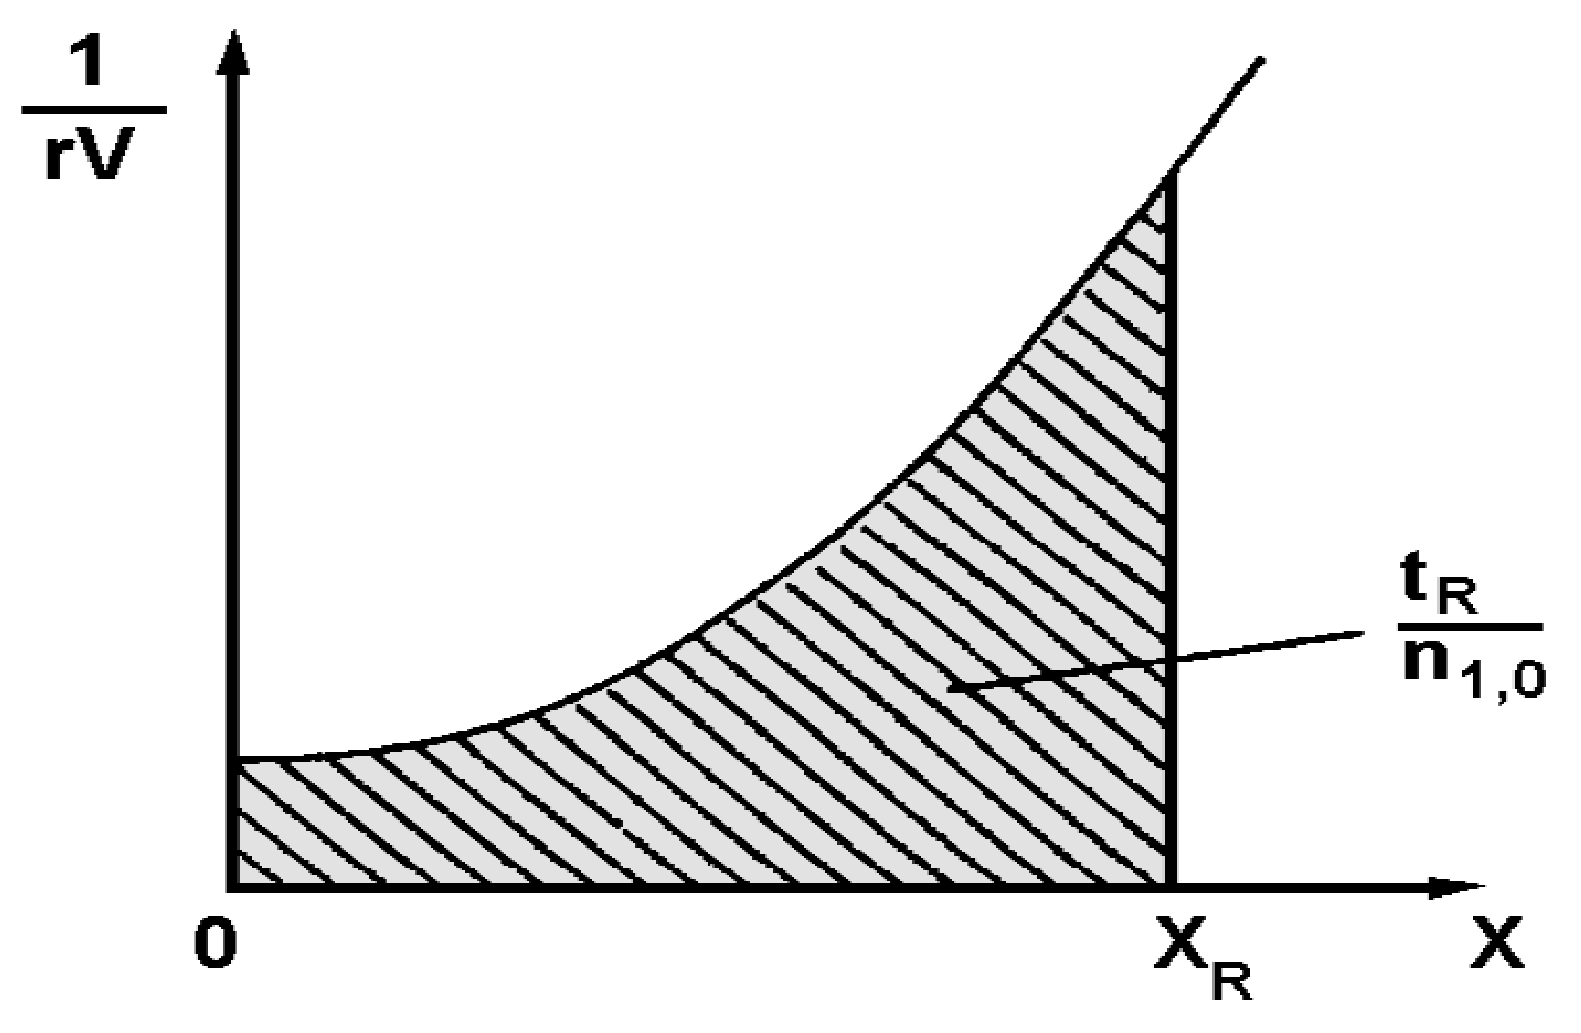
\includegraphics[width=80mm]{images/reaktionszeit.eps}
\end{figure}

\subsection{Ideales Str�mungsrohr (PFTR)}
Es entf�llt der Term f�r Dispersion.\\
Massenbilanz:
\[ \fbox{$\displaystyle \frac{\partial c_i}{\partial t}=-\frac{\partial\left(c_iu\right)}{\partial z}+\sum_j\nu_{ij}r_j$} \]
�blicherweise {\it station�rer} Betrieb $\rightarrow$ $\frac{dc_i}{dt}=0$\\
W�rmebilanz:
\[ \fbox{$\displaystyle \underbrace{\frac{dT}{dz}}_{\mbox{Konvektion}}=\frac{1}{u\rho c_p}\underbrace{\left(\sum_{j}\left(-\Delta H_j\right)r_j\right.}_{\mbox{W�rmequelle/-senke}}-\underbrace{\left.k_W\frac{A}{V}\left(T-T_K\right)\right)}_{\mbox{W�rmetransport}}$} \]
Beim adiabaten Str�mungsrohr entf�llt der W�rmetransport durch die Wand (einzige W�rmever�nderung durch Reaktion).
F�r eine einzelne Reaktion folgt durch Verkn�pfung mit dem Umsatz und Einf�hrung der adiabaten Temperaturerh�hung $\Delta T_{ad}$
\[ \fbox{$\displaystyle dT=\underbrace{\frac{c_{1,0}\left(-\Delta H_R\right)}{\rho_0\cdot \bar c_p}}_{\Delta T_{ad}}dX=\Delta T_{ad}dX$} \]
Adiabate Trajektorie:\\
\[ X=\frac{T-T_0}{\Delta T_{ad}} \]
\subsection{Verkn�pfung von Masse- und W�rmebilanz im nichtisothermen STR}
Bedingung f�r station�ren Betrieb:
\[ \underbrace{\dot q_{gen}}_{\mbox{W�rmeproduktion}}=\underbrace{\dot q_{rem}}_{\mbox{W�rmeabfuhr}} \]
\begin{figure}[H]
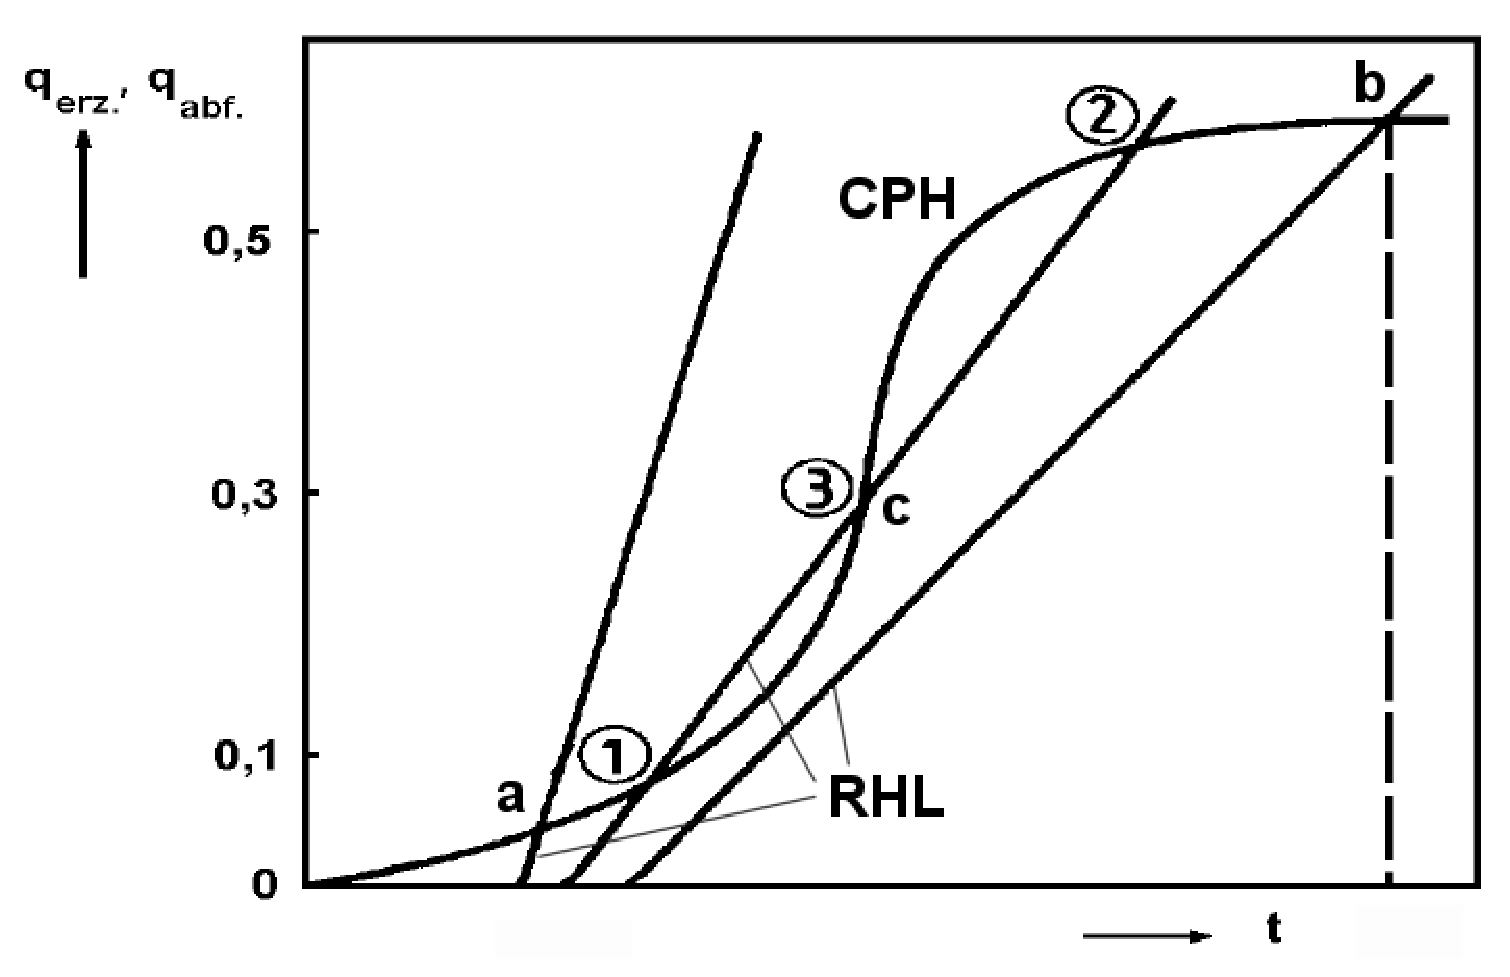
\includegraphics[width=87mm]{images/system.eps}
\end{figure}
CPH: curve of production of heat $\rightarrow$ nichtlinear wegen {\sc Arrhenius}\\
RHL: removal of heat line $\rightarrow$ lineare Funktion der Temperatur\\
$\vartheta=\frac{T}{T_0}$: Temperaturerh�hung im Reaktor (Bulk-/Eingangstemperatur)\\
Drei Betriebsweisen:
\begin{itemize}
\item[a)] {\it gel�schtes System}\\
Temperaturver�nderung verursacht von selbst einen R�ckgang zu einem einzigen stabilen Betriebspunkt.
\item[b)] {\it gez�ndetes System}\\
Wie a) jedoch auf hohem Temperaturniveau
\item[c)] {\it instabiles System}\\
Minimale Temperaturabweichung verursacht Z�nden oder Erl�schen $\rightarrow$ stabiler Betriebspunkt stellt sich ein.
\end{itemize}
Instabiler Betriebspunkt wenn:
\[ \fbox{$\displaystyle \frac{d \dot q_{rem}}{d\vartheta}<\frac{d \dot q_{gen}}{d\vartheta}$} \]
Analoge Darstellung ist im $X-T$-Diagramm m�glich: hier sind RHL's parallel. Ums�tze im instabiler Bereich k�nnen nicht erreicht werden.


\section{Reale Reaktoren}
\subsection{Verweilzeitverteilung}

\end{document}
